% $Header$
% MBDyn (C) is a multibody analysis code.
% http://www.mbdyn.org
%
% Copyright (C) 1996-2007
%
% Pierangelo Masarati  <masarati@aero.polimi.it>
%
% Dipartimento di Ingegneria Aerospaziale - Politecnico di Milano
% via La Masa, 34 - 20156 Milano, Italy
% http://www.aero.polimi.it
%
% Changing this copyright notice is forbidden.
%
% This program is free software; you can redistribute it and/or modify
% it under the terms of the GNU General Public License as published by
% the Free Software Foundation (version 2 of the License).
% 
%
% This program is distributed in the hope that it will be useful,
% but WITHOUT ANY WARRANTY; without even the implied warranty of
% MERCHANTABILITY or FITNESS FOR A PARTICULAR PURPOSE.  See the
% GNU General Public License for more details.
%
% You should have received a copy of the GNU General Public License
% along with this program; if not, write to the Free Software
% Foundation, Inc., 59 Temple Place, Suite 330, Boston, MA  02111-1307  USA
%
% Copyright (C) 2007
%
% Marco Morandini

\chapter{Elements}\label{sec:ELEMENTS}
The \kw{elements} section is enclosed in the cards:
\begin{verbatim}
    begin: elements;
        ...
    end: elements;
\end{verbatim}
Every element card has the following format:
\begin{verbatim}
    <card> ::= <elem_type> : <arglist>
               [ , output , { yes | no } ] ;
\end{verbatim}
where \kw{elem\_type} is one of the following:
\begin{itemize}
\item \kw{aerodynamic beam}
\item \kw{aerodynamic body}
\item \kw{air properties}
\item \kw{automatic structural}
\item \kw{beam}
\item \kw{bind}
\item \kw{body}
\item \kw{bulk}
\item \kw{couple}
\item \kw{electric}
\item \kw{force}
\item \kw{genel}
\item \kw{gravity}
\item \kw{hydraulic}
\item \kw{joint}
\item \kw{loadable}
\item \kw{rotor}
\item \kw{RTAI output}
\item \kw{Miscellaneous}
\end{itemize}
in case of elements that can be instantiated only once, like
the \kw{gravity} or the \kw{air properties} elements, the \kw{arglist}
doesn't contain any label; otherwise, a label is expected first, to allow 
for checks on duplicated elements, namely: 
\begin{verbatim}
    <arglist> ::= <label> , <normal_arglist>
\end{verbatim}
The data manager reads the element type and the label and checks for
duplication. If the element is not defined yet, the proper read function is
called, which parses the rest of the card and constructs the element.
The elements are read as follows.



\section{Aerodynamic Body and Aerodynamic Beam Elements}
These elements share the description of the aerodynamics; the former assumes
the aerodynamic surface to be rigid, and takes its configuration from a
single node, while the latter relies on a three-node beam and uses the
same interpolation functions of the beam to compute the configuration 
at an arbitrary point.
The \kw{aerodynamic body} input format is:
\begin{verbatim}
    <normal_arglist> ::= <node_label> 
        [ , rotor , <rotor_label> ] ,
        (Vec3)              <relative_surface_offset> , 
        (OrientationMatrix) <relative_surface_orientation> ,
        (scalar)            <surface_span> ,
        (shape_1D)          <surface_chord> ,
        (shape_1D)          <surface_aerodynamic_center> ,
        (shape_1D)          <surface_b_c_point> ,
        (shape_1D)          <surface_twist> ,
                            <integration_points>
        [ , control , (drive_caller) <control_drive> ] 
        [ , <airfoil_data> ]
        [ , unsteady , { bielawa } ]
\end{verbatim}
The \kw{aerodynamic beam} input format is:
\begin{verbatim}
    <normal_arglist> ::= <beam_label> 
        [ , rotor , <rotor_label> ] ,
        (Vec3)              <relative_surface_offset_1> ,       
        (OrientationMatrix) <relative_surface_orientation_1> ,
        (Vec3)              <relative_surface_offset_2> ,
        (OrientationMatrix) <relative_surface_orientation_2> ,
        (Vec3)              <relative_surface_offset_3> ,       
        (OrientationMatrix) <relative_surface_orientation_3> ,
        (shape_1D)          <surface_chord> ,
        (shape_1D)          <surface_aerodynamic_center> ,
        (shape_1D)          <surface_b_c_point> ,
        (shape_1D)          <surface_twist> ,
                            <integration_points>
        [ , control , (drive_caller) <control_drive> ] 
        [ , <airfoil_data> ]
        [ , unsteady , { bielawa } ]
\end{verbatim}
where
\begin{verbatim}
    <airfoil_data> ::= { naca 0012 | rae 9671 | c81 , <c81_data> }
\end{verbatim}
and
\begin{verbatim}
    <c81_data> ::= <c81_label> 

    <c81_data> ::= multiple , <airfoil_number> ,
        <c81_label> , <end_point>
        [ ... ]

    <c81_data> ::= interpolated, <airfoil_number> ,
        <c81_label> , <position>
        [ ... ]
\end{verbatim}
The field \kw{rotor} instructs the element that it is linked to a 
\kw{rotor} element; this means that it can get information about the
induced velocity and should supply information about the forces it generates.
An arbitrary configuration and offset is allowed for both elements with
respect to the nodes they are linked to. 
This means that the aerodynamic beam offsets refer to the position of the nodes,
and have nothing to do with offsets related to the structural beam element.
The \kw{shape} entities are used to compute the physical chord,
aerodynamic center, velocity measurement point (the point where the
kinematic boundary conditions are evaluated) and twist as functions 
of the dimensionless abscissa along the span.
The span of the \kw{aerodynamic body} element is set by the user; the
center-span of the element is assumed to be the end of the offset vector.
The span of the \kw{aerodynamic beam} is computed based on the end of the
offset vectors related to nodes 1, 3.
The aerodynamic center and the velocity measurement points are measured
relative to the centerline of the elements, that is the line in direction 3
of the local frame from the end of the offset vector.
This line is assumed to be at the 25\% of the airfoil chord when steady
aerodynamic coefficients are used (\kw{unsteady\_flag} = 0).
The direction 1 is assumed to be the ``reference'' line of the airfoil, 
from the trailing edge to the leading edge (points ``forward''),
while direction 2 is normal to the other two and goes from the lower 
to the upper side of the airfoil (points ``up''). 
Figure~\ref{fig:AIRFOIL} shows the arrangement of the airfoil geometry 
and properties.

\begin{figure}[h]
  \centering
    %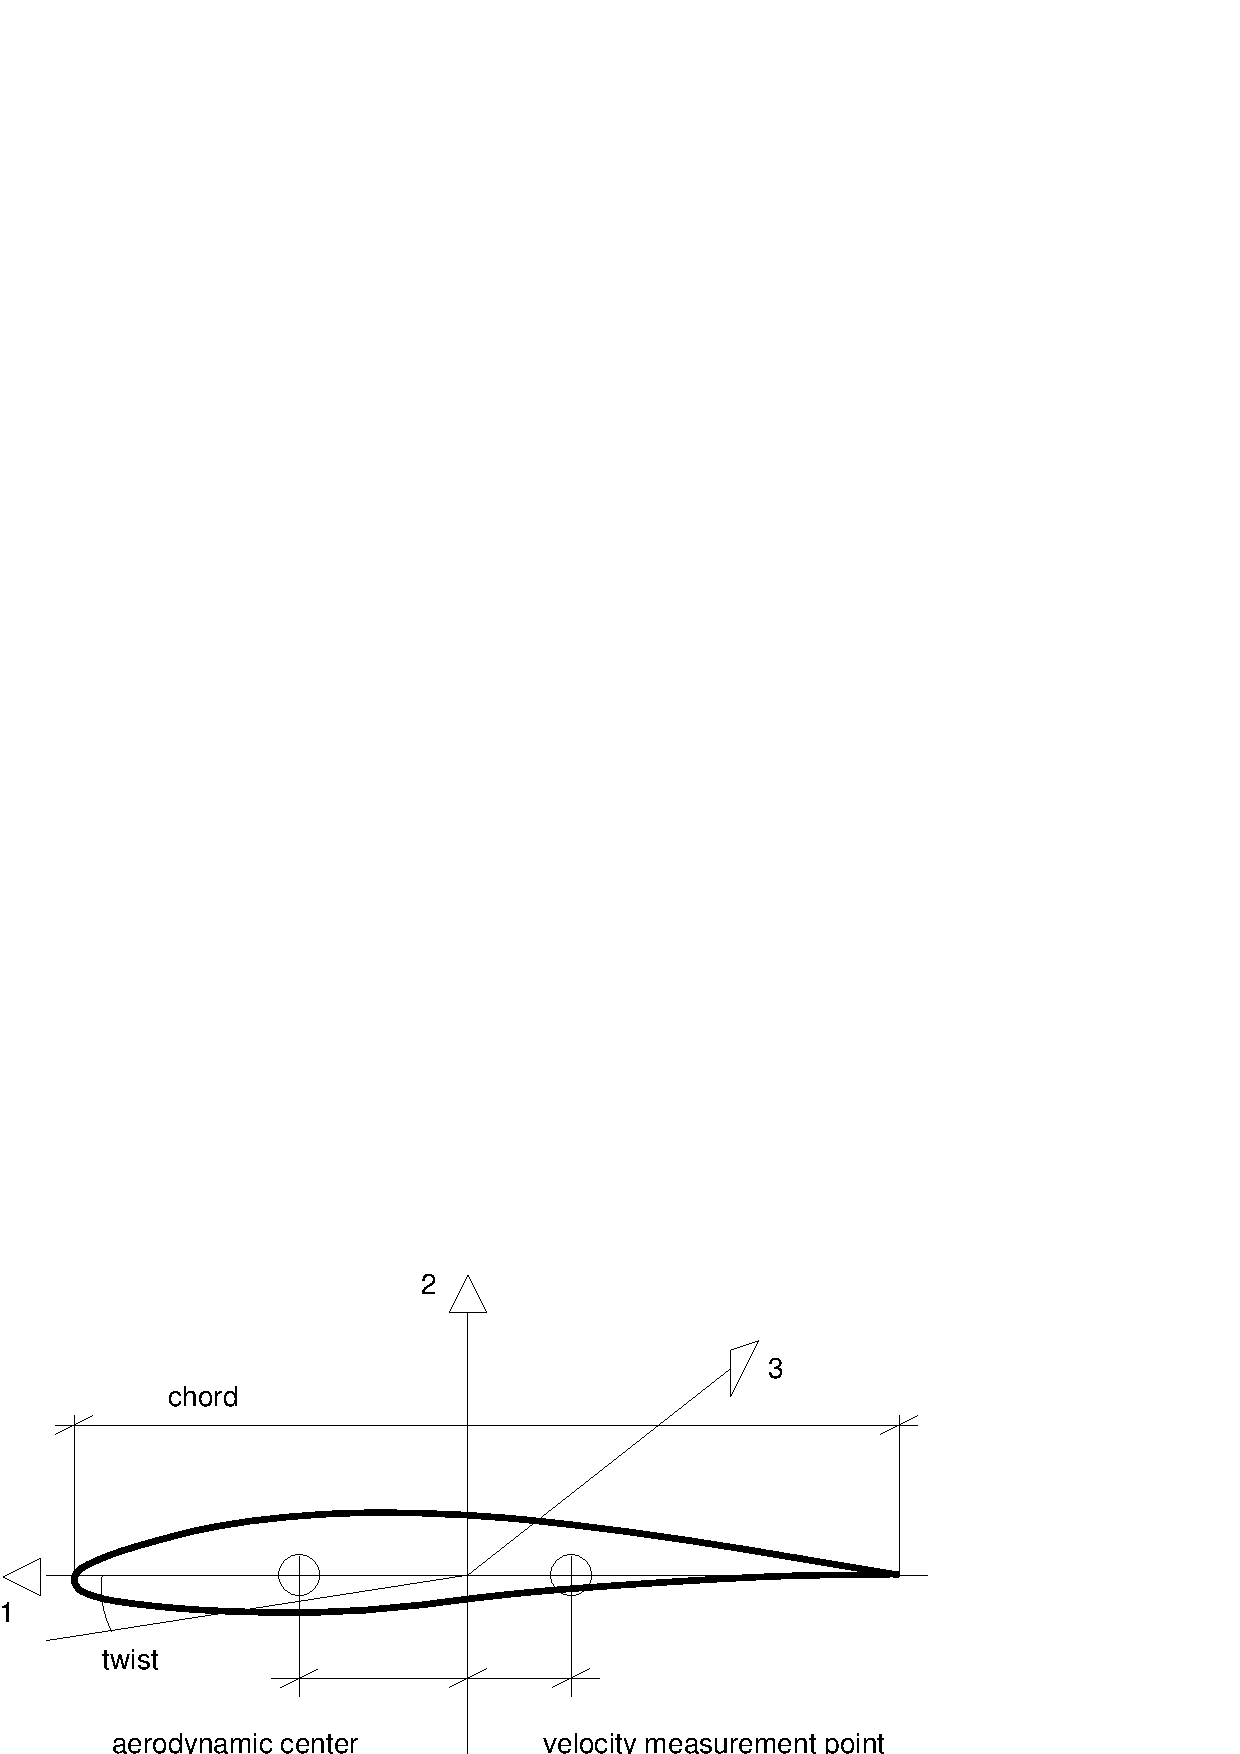
\includegraphics[width=80mm]{airfoil.pdf}
    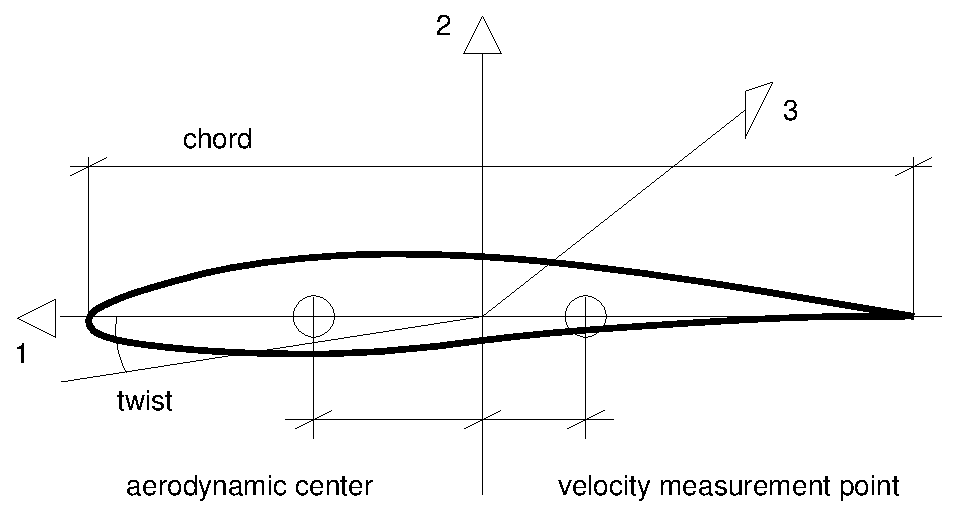
\includegraphics[width=80mm]{airfoil.eps}
  \caption{Airfoil geometry}\label{fig:AIRFOIL}
\end{figure}

The \kw{airfoil\_data} defaults to a built-in NACA 0012 semi-analytical
model (FIXME: the unsteady correction is buggy; use the \kw{c81} 
mode instead).

The \kw{multiple} mode of the c81 data allows to specify
more than one airfoil for an aerodynamic element; the transition
between airfoils is sharp.
The integer \kw{airfoil\_number} indicates how many airfoils are expected;
the real \kw{end\_point} indicates where the influence zone for that
airfoil ends, expressed in terms of a non-dimensional abscissa spanning 
$\plbr{-1,1}$ along the reference line, roughly along axis 3 
of the aerodynamic reference frame; \kw{end\_point} must not lie outside
the element.
So, for example, if airfoil NACA 0015 is used in the leftmost part
of an element up to 1/4 span, NACA 0012 is used from 1/4 to 3/4 span,
and NACA 0009 is used in the remaining rightmost 1/4, the syntax is:
\begin{verbatim}
    set: integer naca0015 = 15;
    set: integer naca0012 = 12;
    set: integer naca0009 = 9;
    c81 data: naca0015, "naca0015.c81";
    c81 data: naca0012, "naca0012.c81";
    c81 data: naca0009, "naca0009.c81";
    # beginning of aerodynamic element definition...
        multiple, 3,
            naca0015, -0.5,    # from -1.0 to -0.5
            naca0012,  0.5,    # from -0.5 to  0.5
            naca0009,  1.0,    # from  0.5 to  1.0
    # ...rest of aerodynamic element definition
\end{verbatim}

The \kw{interpolated} mode of the c81 data allows to specify 
a smooth transition between different airfoils inside an element.
The interpolation occurs at the integration points where the
aerodynamic data is required, and it is performed once for all
at the beginning of the analysis.
Since this operation is time consuming, and essentially unnecessary,
the interpolated data can be generated once for all with the utility
\kw{util/c81merge} once the position of the integration point is known,
and the \kw{multiple} mode can be used to directly provide
the interpolated data to the aerodynamic element.

\noindent
\emph{FIXME: not implemented yet}


\subsection{Output}
Aerodynamic elements, both bodies and beams, write their output with file
extension \kw{.aer}; for each time step the required elements are output.
Three different formats are available; the format can be selected only at
compile time, and it must be the same for all the elements. 

\noindent
\emph{Note: eventually it will freeze; if all the output formats will be
maintained, they will be made selectable at run-time.}

\noindent
In any case the label of the element is output first.

\subsubsection{Node}
The format is:
\begin{itemize}
    \item the label of the node
    \item the three components of the force applied to the node
    \item the three components of the couple applied to the node
\end{itemize}
When an \kw{aerodynamic beam} is considered, the output is repeated 
for each node the element is attached to.

\subsubsection{Forces at Gauss points}
The output refers to each Gauss integration point; the format is:
\begin{itemize}
    \item the direction of the wind velocity relative to the element frame
    \item the lift,
    \item the drag,
    \item and the aerodynamic moment per unit length
\end{itemize}
When an \kw{aerodynamic beam} is considered, the output 
is repeated for each portion of beam.

\subsubsection{Coefficients at Gauss points}
The output refers to each Gauss integration point; the format is:
\begin{itemize}
    \item the local incidence
    \item the local yaw angle
    \item the local Mach number
    \item the lift,
    \item the drag,
    \item and the aerodynamic moment coefficient
\end{itemize}
When an \kw{aerodynamic beam} is considered, the output 
is repeated for each portion of the beam.



\section{Aeromodal Element}
\emph{Note: prepared by Alessandro Scotti.}

\noindent
This element is used to model an aerodynamic modal element,
i.e.\ an unsteady aerodynamic model that inherits the structural 
motion from a  \htmlref{\kw{modal}}{sec:EL:STRUCT:JOINT:MODAL} element
Its definition is very similar to that of the pure modal element, 
but it also includes some data representing unsteady aerodynamics 
in the time domain trough the residualization matrices.
This element is defined as follows:
\begin{verbatim}
    <joint_type> ::= aeromodal
    <joint_arglist> ::= <label> , 
        <modal node> ,  
        <reference modal joint> ,
        (Mat3x3)<orientation> ,
        <reference chord> ,
        <number of aerodynamic states> ,
        <state space modal matrices file>
\end{verbatim}
With this formulation, anytime an aeromodal element is defined, 
the user needs to declare the number of modal aerodynamic elements 
in use in the \kw{control data} section.
An \htmlref{\kw{air properties}}{sec:EL:AERO:AIRPORPERTIES}
card definition is also required. 
The \kw{.fea} file includes the state space model in form 
of matrices $A$, $B$, $C$, $D_0$, $D_1$ and $D_2$, according to the representation
\begin{align*}
	\dot{\T{x}} &= \T{A}\T{x} + \T{B}\T{q} \\	
	\T{f} &= q\plbr{\T{C}\T{x} + \T{D}_0 \T{q} + \frac{2V_{\infty}}{c} \T{D}_1 \dot{\T{q}} + \plbr{\frac{2V_{\infty}}{c}}^2 \T{D}_2 \ddot{\T{q}}}
\end{align*}
where $\T{q}$ are the modal variables that describe the structural motion,
and $\T{f}$ are the unsteady aerodynamic forces that apply to the structural
dynamics equations.

The file is formatted as follows:
\begin{verbatim}
    *** MATRIX A
    (<na> x <na> coefficients)
    *** MATRIX B
    (<na> x <ns> coefficients)
    *** MATRIX C
    (<ns> x <na> coefficients)
    *** MATRIX D0
    (<ns> x <ns> coefficients)
    *** MATRIX D1
    (<ns> x <ns> coefficients)
    *** MATRIX D2
    (<ns> x <ns> coefficients)
\end{verbatim}

\noindent
Example:
\begin{verbatim}
    aeromodal: Wing, Wing, Wing,
        eye,
        131.25, 10, "ha145b.fea";
\end{verbatim}
The \kw{aeromodal} element is declared with the label \kw{Wing}.
This element is attached to a modal node, also labeled
with the name \kw{Wing}, and the reference \kw{modal} joint 
it is referred to is named \kw{Wing} as well.
The orientation of the aerodynamic reference with respect 
to the nodal reference is here expressed by the matrix eye.
The aerodynamic element chord is 131.25 (inches!).
This quantity must be consistent with the system chosen to define 
the whole model (S.I., for example; in this case, British Units).
The next field, 10, indicates the number of states needed to use 
the aerodynamic model.
The string \kw{ha145b.fea} is the name of the file that contains
the state space model matrices, obtained with an approximation 
chosen by the user.
In this particular case, a 10 states Pad\'e approximation 
has been chosen.
This example is taken from the Bisplinghoff Ashley Halfman
(BAH) Jet Transport Wing cantilevered wing with modal aerodynamic 
frequency responce, computed by a double-lattice method at Mach 0.0.
Data were extracted from the MSC-NASTRAN aeroelastic example file, 
named \kw{ha145b}, while the aerodynamic state-space fitting 
has been computed using a Pad\'e polynomial approximation
(by Pasinetti \& Mantegazza).
All quantities are expressed in inches and pounds.



\section{Aircraft Instruments}
\begin{verbatim}
    <card> ::= aircraft instruments
    <arglist> ::= <aircraft_node>
        [ , orientation , (Mat3x3)<relative orientation> ]
\end{verbatim}
The \kw{<aircraft\_node>} represents the aircraft; it is assumed
that the ``nose'' of the aircraft is toward the positive $x$ direction
of the node, and the ``top'' of the aircraft is toward the positive 
$z$ direction of the node.
An optional orientation can be added to change the orientation 
of the aircraft with respect to the node.
This is useful, for example, with helicopters, where conventionally
the positive direction of the $x$ axis is nose to tail.

The available measures are accessed during the simulation 
by defining appropriate \kw{parameter} nodes, and by binding
the \kw{aircraft instruments} element private data to the nodes 
by means of the \kw{bind} mechanism, or directly by means
of the 
\hyperref{\kw{element} drive}{\kw{element} drive (see Section~}{)}{sec:DRIVE-ELEMENT}.

\paragraph{Private Data}
The following data is available:
\begin{itemize}
\item \kw{"airspeed"} the airspeed as seen by the reference 
	point on the aircraft, i.e. the combination 
	of the airstream speed and of the node speed
\item \kw{"groundspeed"} the absolute value of the projection
	of the node speed in the $xy$ plane.
\item \kw{"altitude"} the $z$ component of the node position
\item \kw{"attitude"} $\arctan\plbr{r_{31}, r_{11}}$
	(FIXME: better $\arcsin\plbr{r_{31}}$?)
\item \kw{"bank"} $\arctan\plbr{r_{32}, r_{22}}$
	(FIXME: better $\arcsin\plbr{r_{32}}$?)
\item \kw{"turn"} (not available yet)
\item \kw{"slip"} (not available yet)
\item \kw{"verticalspeed"} the $z$ component of the node velocity
\item \kw{"angleofattack"} the angle between the $z$ 
\item \kw{"heading"} the angle between the $x$ axis of the aircraft 
	and the ``north'' (the global $x$ axis) about the global $z$ axis;
	note: heading wraps about South
	(+180 deg from East, -180 deg from West).
\end{itemize}

\noindent
\emph{Note: this element is eXperimental.}




\section{Air Properties Element}\label{sec:EL:AERO:AIRPORPERTIES}
The properties of the airstream are made of the physical properties
of the air plus the description of the airstream velocity direction
and amplitude.
The former can be expressed in different forms, while the latter
are based on three-dimensional vectors which depend on multipliers.
\begin{verbatim}
    <arglist> ::= {
        (drive_caller) <air_density> , (scalar) <sound_speed> 
        | std , { { SI | British }
            [ , temperature deviation , <delta T> ]
            | <p0> , (drive_caller) <rho0> ,
            <T0> , <dT/dz> , <R> , <g0> , <z1> , <z2>
        } [ , reference altitude, <z0> ]
    } , (Vec3_tpl_drive_caller) <air_speed>
    [ , gust , <gust_model> ]
\end{verbatim}
The first form consists in the bare input of the air density,
in form of a drive caller, and of the sound celerity, e.g.:
\begin{verbatim}
    air properties: 1.225, 340.,
        1.,0.,0., 150.;
\end{verbatim}
The second form uses standard air properties, both in the
international system (SI) or in British units, possibly
with a temperature deviation and an altitude offset, e.g.:
\begin{verbatim}
    air properties: std, SI, temperature deviation, -55,
        reference altitude, 1000.,
        1.,0.,0., 150.;
\end{verbatim}
where standard properties in SI are used, with a temperature
deviation of -55 K and a reference altitude of 1000 m.
The air properties are computed based on the Z position of the
point where the air properties are requested (plus the optional
altitude offset).
The last possibility lets the user input all the parameters
required to compute the air properties based on the Z position
of the point where they are requested, namely the reference
pressure \kw{p0}, the reference density \kw{rho0},
the reference temperature \kw{T0}, the initial temperature
gradient \kw{dT/dz}, the gas constant \kw{R}, the
initial gravity acceleration \kw{g0}, the bottom and top
altitudes of the null temperature gradient region \kw{z1} and
\kw{z2}; e.g., for SI units:
\begin{verbatim}
    air properties: std,
        101325.,       /* Pa */
        1.2250,        /* kg/m^3 */
        288.16,        /* K */
        -6.5e-3,       /* K/m */
        287.,          /* J/kgK */
        9.81,          /* m/s^2 */
        11000.,        /* m */
        25000.,        /* m */
        temperature deviation, -55,
        reference altitude, 1000.,
        1.,0.,0., 150.;
\end{verbatim}
The asymptotic air properties are characterized by the 3D template drive 
of the air speed, in the global reference frame.
If the optional \kw{gust} keyword is used, a gust model can be added.
Note that a very elementary gust model, represented by a uniform change
in airstream speed and direction can be implemented by using
a time-dependent airstream drive.
A more sophisticated model is currently available, and provisions are
made to allow four-dimensional gust profiles, dependent on time
and position.
The syntax is:
\begin{verbatim}
    <gust_model> ::= front 1D ,
        (Vec3) <front_direction> ,
        (Vec3) <perturbation_direction> ,
        (scalar) <front_velocity> ,
        (drive_caller) <front_profile>
\end{verbatim}
This model consists in a uniform front, defined as
\begin{displaymath}
	\T{v}\plbr{\T{x}, t} = \T{n} g\plbr{\T{f} \cdot \T{x} + V_{ref} \cdot t}
\end{displaymath}
where
\begin{itemize}
\item $\T{v}$ is the velocity perturbation;
\item $\T{x}$ is the position of the point whose airstream velocity
is being computed;
\item $t$ is the current time;
\item $\T{n}$ is the unit vector \kw{perturbation\_direction} 
that defines the direction of the velocity perturbation;
\item $g\plbr{\cdot}$ is the function \kw{front\_profile} 
that defines the gust profile;
\item $\T{f}$ is the unit vector \kw{front\_direction} 
that defines the direction of propagation of the front;
\item $V_{ref}$ is the velocity \kw{front\_velocity} 
of propagation of the front in direction $\T{f}$.
\end{itemize}
As an example, a transverse cosine-shaped gust, with a wavelength of 100 m
and a peak velocity of 5 m/s moving downstream at the airstream speed,
100 m/s, in standard air, is presented:
\begin{verbatim}
    set: real waveLength = 100.; # m
    set: real V_inf = 100.;      # m/s
    set: real V_g = 5.;          # m/s
    air properties: std, SI,
        1.,0.,0., const, V_inf,  # reference airstream along X
        gust, front 1D,
            1.,0.,0.,            # front moving along X
            0.,0.,1.,            # gust along Z
            V_inf,               # front moving at V_inf
            cosine, 0., pi/waveLength, V_g/2., one, 0.;
\end{verbatim}

\subsection{Output}
The output occurs in the \kw{.air} file, which contains:
\begin{itemize}
\item a fake label, always set to 0
\item the air density
\item the sound celerity
\item the three components of the reference air speed
with respect to the inertial reference frame
\end{itemize}



\section{Automatic structural}
The so called \kw{automatic structural} element is automatically generated
when a dynamic structural node is instantiated.
As such, when defined in the \kw{elements} block,
the element already exists.
The only reason to repeat its definition is to modify the values
of the momentum and of the momenta moment, and to initialize
their derivatives.
The label must match that of the node it refers to.
\begin{verbatim}
    <element_type> ::= beam3
    <normal_arglist> ::=
        (Vec3) <momentum> ,
        (Vec3) <momenta_moment> ,
        (Vec3) <momentum_derivative> ,
        (Vec3) <momenta_moment_derivative>
\end{verbatim}
All the provided values are recomputed during the initial derivatives phase,
so they should be intended as initial values for the Newton iteration.
In general, there is no need to provide this data; they can speed up
initial convergence in case of systems that are not at rest in the initial
configuration, with kinematic constraints that strongly affect
the motion.

\paragraph{Private Data}
The following data is available:
\begin{enumerate}
\item \kw{"beta[1]"} momentum in global direction 1
\item \kw{"beta[2]"} momentum in global direction 2
\item \kw{"beta[3]"} momentum in global direction 3
\item \kw{"gamma[1]"} momenta moment in global direction 1
\item \kw{"gamma[2]"} momenta moment in global direction 2
\item \kw{"gamma[3]"} momenta moment in global direction 3
\item \kw{"betaP[1]"} momentum derivative in global direction 1
\item \kw{"betaP[2]"} momentum derivative in global direction 2
\item \kw{"betaP[3]"} momentum derivative in global direction 3
\item \kw{"gammaP[1]"} momenta moment derivative in global direction 1
\item \kw{"gammaP[2]"} momenta moment derivative in global direction 2
\item \kw{"gammaP[3]"} momenta moment derivative in global direction 3
\end{enumerate}





\section{Beam Element}
The family of finite volume beam elements implemented in MBDyn
allows to model slender deformable structural components 
with a high level of flexibility.

\noindent
The beam is defined by a reference line and by a manifold
of orientations attached to the line.
It is assumed that the direction 1 of the orientations lies along
the reference line, but it is not strictly required to be tangent
to it even in the reference configuration.

\noindent
The beam element is defined by its nodes; currently, 2 and 3 node 
beam elements are implemented.
Each node of the beam is related to a \kw{structural node} by an offset
and a relative orientation, to provide topological flexibility.
The beam element is modeled by means of an original Finite Volume approach
\cite{FV-AIAA}, which computes the internal forces as functions 
of the straining of the reference line and orientation at selected points
along the line itself, called \emph{evaluation points},
which lie somewhere between two pairs of beam nodes.
At each evaluation point, a 6D constitutive law must be defined,
which defines the relationship between the strains, the curvatures
of the beam and their time derivatives
and the internal forces and moments at the evaluation points.
The strains and curvatures and their time derivatives are obtained 
from the nodal positions and orientations by differentiating
the interpolation functions.
The 6D constitutive laws are defined as
\begin{displaymath}
	\cubr{\cvvect{
		F_x \\
		F_y \\
		F_z \\
		M_x \\
		M_y \\
		M_z
	}} = \T{f}\plbr{
		\cubr{\cvvect{
			\varepsilon_x \\
			\gamma_y \\
			\gamma_z \\
			\kappa_x \\
			\kappa_y \\
			\kappa_z
		}},
		\cubr{\cvvect{
			\dot{\varepsilon}_x \\
			\dot{\gamma}_y \\
			\dot{\gamma}_z \\
			\dot{\kappa}_x \\
			\dot{\kappa}_y \\
			\dot{\kappa}_z
		}}
	}
\end{displaymath}
where, if the convention of using $x$ as beam axis is followed:
\begin{itemize}
\item $F_x$ is the axial force component;
\item $F_y$ and $F_z$ are the shear force components;
\item $M_x$ is the torsional moment component;
\item $M_y$ and $M_z$ are the bending moment components;
\item $\varepsilon_x$ is the axial strain component;
\item $\gamma_y$ and $\gamma_z$ are the shear strain components;
\item $\kappa_x$ is the torsional curvature component;
\item $\kappa_y$ and $\kappa_z$ are the bending curvature component;
\item $\T{f}$ is an arbitrary function that defines the constitutive law.
\end{itemize}



\subsection{Beam Section Constitutive Law}
Typically, linear elastic or viscoelastic constitutive laws are used,
although one may want to implement specific nonlinear elastic
or elastic-plastic constitutive laws.



\subsubsection{Beam Section Characterization}
MBDyn allows the broadest generality in defining what a linear elastic 
constitutive law contains, since the entire $6\times{6}$ constitutive
matrix can be input.
This means that internal forces and couples can be arbitrarily related
to generalized strains and curvatures.
However, to make sense, a constitutive matrix at the section level,
must satisfy some constraints, e.g.\ it is expected to be symmetric, 
although this is not strictly enforced by the code.

However, most of the info about the extra-diagonal terms 
of the stiffness matrix are not usually available.
One easy way to work this around is to resort to any so-called
composite beam section characterization analysis available 
in the literature.
For details, the reader is referred to \cite{HODGES-REVIEW90} 
for a review of the topic, to \cite{ANBA-GIAVOTTO-83}
for an early work on the subject, and to \cite{MASARATI-2001}
for a recent review of the original formulation.


\subsubsection{Disclaimer}
The following paragraphs are intended as a means to help users
preparing data for MBDyn models in a consistent manner.
By no means they indicate that the beam section stiffness properties
must be provided in a specific reference frame.
On the contrary, MBDyn allows as much generality as possible,
and actually the variety of choices is redundant, since equivalent
properties can be input in different ways.
This is intended to allow the code to suit the user's needs
regardless of the original format of the input data.
As such, all the transformations reported in the following 
are only intended as suggestions and should not be taken literally.
For instance, rotations and transportation of reference points
could be reversed, changing the values of the offsets, without
affecting the final result.
The most important aspect of MBDyn notion of beam section properties
is that the reference point and orientation, although arbitrary,
must be unique, and the common notions of center of axial strain,
shear center (and center of mass) have no special meaning.



\subsubsection{Equivalent $6\times6$ Section of Isotropic Beam}
When an isotropic beam section is considered, the $6\times$ 
constitutive matrix, referred to an arbitrary point in the section,
with an arbitrary orientation, can always be written in terms 
of elementary stiffness and geometrical properties.
These are the properties that are usually available in tabular form
either from simplified beam section analysis or by experiments.
A sketch of a generic section is shown
in Figure~\ref{fig:EL:BEAM:SECTION},
where the arbitrary reference frame indicated by axes 
$x$, $y$ and $z$ originates from an arbitrary reference point
on the section.

Isotropic uniform beam sections allow to group the internal forces 
and couples in two sets, together with their conjugated generalized 
strains:
those related to shear stress and strain, and those related 
to axial stress and strain, as illustrated
in Figure~\ref{fig:EL:BEAM:GROUPS}.
\begin{figure}[h]
\centering
\begin{tabular}{c|c|c|c|c|c|c|}
	&
		$\varepsilon_x$ &
		$\gamma_y$ &
		$\gamma_z$ &
		$\kappa_x$ &
		$\kappa_y$ &
		$\kappa_z$ \\
	\hline
	$F_x$ & A &   &   &   & A & A \\
	\hline
	$F_y$ &   & S & S & S &   &   \\
	\hline
	$F_z$ &   & S & S & S &   &   \\
	\hline
	$M_x$ &   & S & S & S &   &   \\
	\hline
	$M_y$ & A &   &   &   & A & A \\
	\hline
	$M_z$ & A &   &   &   & A & A \\
	\hline
\end{tabular}
\caption{Constitutive coefficients grouping (S: shear, A: axial)}
\label{fig:EL:BEAM:GROUPS}
\end{figure}
There is no direct coupling between the two group, at the section level,
so the corresponding coupling coefficients are always zero.
This is no longer true when material anisotropy must be taken 
into account.

The $3\times3$ sub-blocks can be separately transformed 
in diagonal form by referring the corresponding properties
to appropriate separate points in the beam section, 
and by applying an appropriate rotation about the axis of the beam.



\subsubsection{Axial Stress and Strain Properties}
Consider first the submatrix represented by the coefficients 
marked as A in Figure~\ref{fig:EL:BEAM:GROUPS}, under the assumption 
that it is symmetric, as indicated in Equation~(\ref{eq:EL:BEAM:AXIAL}):
\begin{equation}
	\cubr{\cvvect{
		F_x \\
		M_y \\
		M_z
	}} = \sqbr{\matr{ccc}{
		A_{11} & A_{12} & A_{13} \\
		 & A_{22} & A_{23} \\
		\llk{sym.} & & A_{33}
	}}\cubr{\cvvect{
		\varepsilon_x \\
		\kappa_y \\
		\kappa_z
	}}
	\label{eq:EL:BEAM:AXIAL}
\end{equation}
The transformation of Equation~(\ref{eq:EL:BEAM:AXIAL-TRANSFORM})
moves the point of application of the axial force 
of an arbitrary amount $\cubr{y,z}$ in the beam section, to the point
indicated as $as$ (axial strain) in Figure~\ref{fig:EL:BEAM:SECTION}:
\begin{eqnarray}
	\cubr{\cvvect{
		F_x \\
		M_y \\
		M_z
	}}^*
	& = & \sqbr{T_{\llk{axial}}}\cubr{\cvvect{
		F_x \\
		M_y \\
		M_z
	}}
	\nonumber \\
	& = & \sqbr{\matr{ccc}{
		 1 & 0 & 0 \\
		 z & 1 & 0 \\
		-y & 0 & 1
	}}\cubr{\cvvect{
		F_x \\
		M_y \\
		M_z
	}}
	\label{eq:EL:BEAM:AXIAL-TRANSFORM}
\end{eqnarray}
So the transformed axial block of the constitutive matrix becomes
\begin{eqnarray}
	\cubr{\cvvect{
		F_x \\
		M_y \\
		M_z
	}}^*
	& = & \sqbr{T_{\llk{axial}}}
	\cubr{\cvvect{
		F_x \\
		M_y \\
		M_z
	}}
	\nonumber \\
	& = & \sqbr{T_{\llk{axial}}} \sqbr{A} \sqbr{T_{\llk{axial}}}^T
	\cubr{\cvvect{
		\varepsilon_x \\
		\kappa_y \\
		\kappa_z
	}}^*
	\label{eq:EL:BEAM:AXIAL-TRANSFORMED}
	\\
	& = &
	\sqbr{\matr{ccc}{
		A_{11} & A_{12} + z A_{11} & A_{13} - y A_{11} \\
		& A_{22} + 2 z A_{12} + z^2 A_{11} & 
			A_{23} + z A_{13} - y A_{12} - yz A_{11} \\
		\llk{sym.} &  & A_{33} - 2 y A_{13} + y^2 A_{13}
	}}\cubr{\cvvect{
		\varepsilon_x \\
		\kappa_y \\
		\kappa_z
	}}^*
	\nonumber
\end{eqnarray}
If the position of the point is selected in such a manner 
that the axial force and the bending moment are decoupled, i.e.,
according to the definition of center of axial strain,
\begin{eqnarray*}
	y & = & \frac{A_{13}}{A_{11}} \\
	z & = & -\frac{A_{12}}{A_{11}}
\end{eqnarray*}
the axial block becomes
\begin{eqnarray*}
	\cubr{\cvvect{
		F_x \\
		M_y \\
		M_z
	}}^*
	& = &
	\sqbr{\matr{ccc}{
		A_{11} & 0 & 0 \\
		& A_{22} - A_{12}^2/A_{11} & A_{23} - A_{12}A_{13}/A_{11} \\
		\llk{sym.} &  & A_{33} - A_{13}^2/A_{11}
	}}\cubr{\cvvect{
		\varepsilon_x \\
		\kappa_y \\
		\kappa_z
	}}^*
	\\
	& = &
	\sqbr{\matr{ccc}{
		A_{11}^* & 0 & 0 \\
		& A_{22}^* & A_{23}^* \\
		\llk{sym.} &  & A_{33}^*
	}}\cubr{\cvvect{
		\varepsilon_x \\
		\kappa_y \\
		\kappa_z
	}}^*
\end{eqnarray*}
Now, a rotation about the beam section axis can be applied 
in order to decouple the bending moments:
\begin{eqnarray}
	\cubr{\cvvect{
		F_x \\
		M_y \\
		M_z
	}}^{\dagger}
	& = & \sqbr{R_{\llk{axial}}}\cubr{\cvvect{
		F_x \\
		M_y \\
		M_z
	}}^*
	\nonumber \\
	& = & \sqbr{\matr{ccc}{
		 1 & 0 & 0 \\
		 0 & \cos\alpha & -\sin\alpha \\
		 0 & \sin\alpha & \cos\alpha
	}}\cubr{\cvvect{
		F_x \\
		M_y \\
		M_z
	}}^*
	\label{eq:EL:BEAM:AXIAL-ROTATION}
\end{eqnarray}
The angle that decouples the bending moments is
\begin{equation*}
	\alpha = \frac{1}{2}\llk{atan}\plbr{\frac{2 A_{23}^*}{A_{22}^* - A_{33}^*}}
\end{equation*}
representing a rotation about the beam axis $x$ at point $as$
(axial strain) in Figure~\ref{fig:EL:BEAM:SECTION},
and the resulting coefficients are
\begin{eqnarray}
	EA & = & A_{11} \\
	EJ_y & = & A_{22}^* \cos^2\alpha + A_{33}^* \sin^2\alpha
		- 2 A_{23}^* \sin\alpha \cos\alpha \\
	EJ_z & = & A_{22}^* \sin^2\alpha + A_{33}^* \cos^2\alpha
		+ 2 A_{23}^* \sin\alpha \cos\alpha
\end{eqnarray}
When the axial and bending stiffnesses, and the position 
of the axial strain center and the orientation of the neutral axes
are available, the axial portion of the stiffness matrix 
can be computed by reversing the order of the transformations 
described in
Equations~(\ref{eq:EL:BEAM:AXIAL-TRANSFORM}--\ref{eq:EL:BEAM:AXIAL-ROTATION}),
i.e.:
\begin{equation}
	\sqbr{\matr{ccc}{
		A_{11} & A_{12} & A_{13} \\
		& A_{22} & A_{23} \\
		\llk{sym.} & & A_{33}
	}} = \sqbr{T_{\llk{axial}}}^{-1} \sqbr{R_{\llk{axial}}}^T \sqbr{\matr{ccc}{
		EA & 0 & 0 \\
		0 & EJ_y & 0 \\
		0 & 0 & EJ_z
	}} \sqbr{R_{\llk{axial}}} \sqbr{T_{\llk{axial}}}^{-T}
	\label{eq:EL:BEAM:AXIAL-TRANSFORM-REVERSED}
\end{equation}
This expression implies that the stiffness properties are referred
to an arbitrary point at $\cubr{-y,-z}$ from the axial strain center,
after that they are rotated into the section reference frame, 
i.e.\ by an amount $-\alpha$.
The resulting coefficients are
\begin{eqnarray*}
	A_{11} & = & EA \\
	A_{12} & = & -z EA \\
	A_{13} & = & y EA \\
	A_{22} & = & EJ_y \cos^2\alpha + EJ_z \sin^2\alpha + z^2 EA \\
	A_{23} & = & \plbr{EJ_z - EJ_y} \sin\alpha\cos\alpha - y z EA \\
	A_{33} & = & EJ_z \cos^2\alpha + EJ_y \sin^2\alpha + y^2 EA
\end{eqnarray*}



\subsubsection{Shear Stress and Strain Properties}
Consider now the submatrix represented by the coefficients 
marked as S in Figure~\ref{fig:EL:BEAM:GROUPS}, under the assumption 
that it is symmetric, as indicated in Equation~(\ref{eq:EL:BEAM:SHEAR}):
\begin{equation}
	\cubr{\cvvect{
		F_y \\
		F_z \\
		M_x
	}} = \sqbr{\matr{ccc}{
		S_{11} & S_{12} & S_{13} \\
		 & S_{22} & S_{23} \\
		\llk{sym.} & & S_{33}
	}}\cubr{\cvvect{
		\gamma_y \\
		\gamma_z \\
		\kappa_x
	}}
	\label{eq:EL:BEAM:SHEAR}
\end{equation}
The orientation of the shear force components about the section axis
can be selected in order to decouple them; by applying the transformation
\begin{eqnarray}
	\cubr{\cvvect{
		F_y \\
		F_z \\
		M_x
	}}^{\dagger}
	& = & \sqbr{R_{\llk{axial}}}\cubr{\cvvect{
		F_y \\
		F_z \\
		M_x
	}}^*
	\nonumber \\
	& = & \sqbr{\matr{ccc}{
		\cos\beta & -\sin\beta & 0 \\
		\sin\beta & \cos\beta & 0 \\
		0 & 0 & 1
	}}\cubr{\cvvect{
		F_y \\
		F_z \\
		M_x
	}}^*
	\label{eq:EL:BEAM:SHEAR-ROTATION}
\end{eqnarray}
The angle that decouples the shear forces is
\begin{equation*}
	\beta = \frac{1}{2}\llk{atan}\plbr{\frac{2 S_{12}^*}{S_{22}^* - S_{11}^*}}
\end{equation*}
representing a rotation about the axis $x$ of the beam with respect
to the origin of the initial reference frame as shown 
in Figure~\ref{fig:EL:BEAM:SECTION},
and the resulting coefficients are
\begin{eqnarray}
	GA_y & = & S_{11}^* \cos^2\alpha + S_{22}^* \sin^2\alpha
		- 2 S_{12}^* \sin\alpha \cos\alpha \\
	GA_z & = & S_{11}^* \sin^2\alpha + S_{22}^* \cos^2\alpha
		+ 2 S_{12}^* \sin\alpha \cos\alpha
\end{eqnarray}
the shear block becomes
\begin{eqnarray*}
	\cubr{\cvvect{
		F_y \\
		F_x \\
		M_x
	}}^*
	& = &
	\sqbr{\matr{ccc}{
		GA_y & 0 & S_{13}\cos\beta - S_{23}\sin\beta \\
		& GA_z & S_{13}\sin\beta + S_{23}\cos\beta \\
		\llk{sym.} &  & S_{33}
	}}\cubr{\cvvect{
		\gamma_y \\
		\gamma_z \\
		\kappa_x
	}}^*
	\\
	& = &
	\sqbr{\matr{ccc}{
		GA_y & 0 & S_{13}^* \\
		& GA_z & S_{23}^* \\
		\llk{sym.} &  & S_{33}
	}}\cubr{\cvvect{
		\gamma_y \\
		\gamma_z \\
		\kappa_x
	}}^*
\end{eqnarray*}
The transformation of Equation~(\ref{eq:EL:BEAM:SHEAR-TRANSFORM})
moves the point of application of the shear force 
of an arbitrary amount $\cubr{y,z}$ in the beam section,
with respect to the reference frame rotated by $\beta$ about 
the axis $x$ of the beam, as indicated
in Figure~\ref{fig:EL:BEAM:SECTION}:
\begin{eqnarray}
	\cubr{\cvvect{
		F_y \\
		F_z \\
		M_x
	}}^{\dagger}
	& = & \sqbr{T_{\llk{shear}}}\cubr{\cvvect{
		F_y \\
		F_z \\
		M_x
	}}^*
	\nonumber \\
	& = & \sqbr{\matr{ccc}{
		1 &  0 & 0 \\
		0 &  1 & 0 \\
		z & -y & 1
	}}\cubr{\cvvect{
		F_y \\
		F_z \\
		M_x
	}}^*
	\label{eq:EL:BEAM:SHEAR-TRANSFORM}
\end{eqnarray}
So the transformed shear block of the constitutive matrix becomes
\begin{eqnarray}
	\cubr{\cvvect{
		F_y \\
		F_z \\
		M_x
	}}^{\dagger}
	& = & \sqbr{T_{\llk{shear}}}
	\cubr{\cvvect{
		F_y \\
		F_z \\
		M_x
	}}^*
	\nonumber \\
	& = & \sqbr{T_{\llk{shear}}} \sqbr{A} \sqbr{T_{\llk{shear}}}^T
	\cubr{\cvvect{
		\gamma_y \\
		\gamma_z \\
		\kappa_x
	}}^{\dagger}
	\label{eq:EL:BEAM:SHEAR-TRANSFORMED}
	\\
	& = &
	\sqbr{\matr{ccc}{
		GA_y & 0 & S_{13}^* + z GA_y \\
		& GA_z & S_{23}^* - y GA_z \\
		\llk{sym.} &  & S_{33} - y S_{23}^* + z S_{13}^*
		+z\plbr{S_{13}^* + z GA_y} - y\plbr{S_{23}^* - y GA_z}
	}}\cubr{\cvvect{
		\gamma_y \\
		\gamma_z \\
		\kappa_x
	}}^{\dagger}
	\nonumber
\end{eqnarray}
If the position of the point is selected in such a manner 
that the shear force and the torsional moment are decoupled, i.e.,
according to the definition of center of shear force (the point 
in a beam section where the application of a transverse force
results in no twist)
\begin{eqnarray*}
	y & = & -\frac{S_{13}^*}{GA_y} \\
	z & = & \frac{S_{23}^*}{GA_z}
\end{eqnarray*}
the shear block becomes
\begin{eqnarray*}
	\cubr{\cvvect{
		F_y \\
		F_x \\
		M_x
	}}^{\dagger}
	& = &
	\sqbr{\matr{ccc}{
		GA_y & 0 & 0 \\
		& GA_z & 0 \\
		\llk{sym.} &  & S_{33} - {S_{13}^*}^2/GA_y - {S_{23}^*}^2/GA_z
	}}\cubr{\cvvect{
		\gamma_y \\
		\gamma_z \\
		\kappa_x
	}}^{\dagger}
	\\
	& = &
	\sqbr{\matr{ccc}{
		GA_y & 0 & 0 \\
		& GA_z & 0 \\
		\llk{sym.} &  & GJ
	}}\cubr{\cvvect{
		\gamma_y \\
		\gamma_z \\
		\kappa_x
	}}^{\dagger}
\end{eqnarray*}
When the shear and torsional stiffnesses, and the position 
of the shear strain center and the orientation of the shear axes
are available, the shear portion of the stiffness matrix 
can be computed by reversing the order of the transformations 
described in
Equations~(\ref{eq:EL:BEAM:SHEAR-ROTATION}--\ref{eq:EL:BEAM:SHEAR-TRANSFORM}),
i.e.:
\begin{equation}
	\sqbr{\matr{ccc}{
		S_{11} & S_{12} & S_{13} \\
		& S_{22} & S_{23} \\
		\llk{sym.} & & S_{33}
	}} = \sqbr{R_{\llk{shear}}}^T \sqbr{T_{\llk{shear}}}^{-1} \sqbr{\matr{ccc}{
		GA_y & 0 & 0 \\
		0 & GA_z & 0 \\
		0 & 0 & GJ
	}} \sqbr{T_{\llk{shear}}}^{-T} \sqbr{R_{\llk{shear}}}
	\label{eq:EL:BEAM:SHEAR-TRANSFORM-REVERSED}
\end{equation}
This expression implies that the stiffness properties are referred
to an arbitrary point at $\cubr{-y,-z}$ from the shear center,
in the shear reference frame, followed by a rotation
into the section reference frame by an amount $-\beta$.
The resulting coefficients are
\begin{eqnarray*}
	S_{11} & = & GA_y \cos^2\beta + GA_z \sin^2\beta \\
	S_{12} & = & \plbr{GA_z - GA_y} \sin\beta\cos\beta \\
	S_{13} & = & y GA_z \sin\beta - z GA_y \cos\beta \\
	S_{22} & = & GA_z \cos^2\beta + GA_y \sin^2\beta \\
	S_{23} & = & y GA_z \cos\beta + z GA_y \sin\beta \\
	S_{33} & = & GJ + z^2 GA_y + y^2 GA_z
\end{eqnarray*}
Note that the order of the rotation and reference point transportation 
is reversed with respect to the axial properties; this is mostly done
for convenience in computing the coefficients, because the opposite
would result in more complicated formulas; however, their development
the other way 'round is straightforward.

\begin{figure}
\centering
\psfrag{alpha}{\hspace{0cm}\large $\alpha$}
\psfrag{beta}{\hspace{0cm}\large $\beta$}
\psfrag{sc}{\hspace{0cm}\large s.c.}
\psfrag{a.s.}{\hspace{0cm}\large a.s.}
\psfrag{x}{\hspace{0cm}\large $x$}
\psfrag{y}{\hspace{0cm}\large $y$}
\psfrag{z}{\hspace{0cm}\large $z$}
\psfrag{ysc}{\hspace{0cm}\large $y_{sc}$}
\psfrag{zsc}{\hspace{0cm}\large $z_{sc}$}
\psfrag{yas}{\hspace{0cm}\large $y_{as}$}
\psfrag{zas}{\hspace{0cm}\large $z_{as}$}
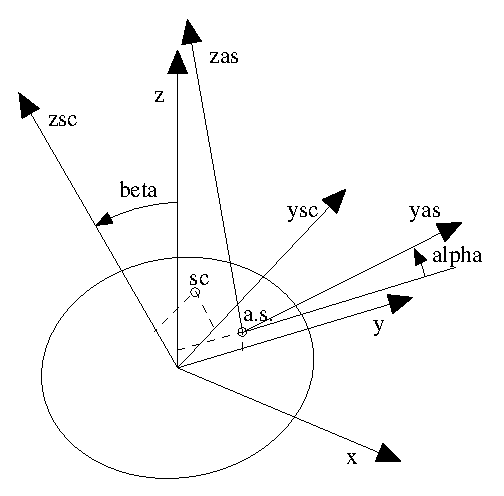
\includegraphics[width=.7\textwidth]{beamsect}
\caption{Beam section}
\label{fig:EL:BEAM:SECTION}
\end{figure}



\subsubsection{Locking Correction for Two-Node Beam}
The three-node finite volume element has been implemented first, 
and uses conventional polynomial parabolic interpolation 
of the nodal displacements and orientations;
the two-node finite volume element has been introduced later.
This latter element presents some shear-locking, which, for linear elastic
constitutive laws, may be overcome by correcting the section stiffness matrix
in a relatively straightforward form:
\begin{equation}\label{eq:2-NODE-BEAM-STIFFNESS}
	\hat{\T{K}} = \plbr{\T{F} + \frac{L^2}{12}\T{T} \T{F} \T{T}^T}^{-1} ,
\end{equation}
where $\T{F}=\T{K}^{-1}$ is the compliance matrix of the section, 
$L$ is the length of the beam, i.e.\ the distance between
the two reference points obtained by adding the optional offset 
to the nodes, and
\begin{displaymath}
	\T{T} \ = \ \sqbr{\matr{cc}{
		\T{0} & \T{e}_x \times{} \\
		\T{0} & \T{0}
	}}
\end{displaymath}
is the ``arm'' matrix that appears in the differential equilibrium equation
\begin{displaymath}
	\T{\vartheta}_{/x} - \T{T}^T\vartheta + \T{f} \ = \ 0 .
\end{displaymath}
There are no provisions to automatically apply the correction 
when defining the constitutive law of the section.
The two-node beam has been reimplemented using a helicoidal interpolation
of the nodal positions and orientations, to improve its capability
to undergo large displacements and relative rotations.
It is activated by using the keyword \kw{hbeam2} instead of \kw{beam2}.
However, to reduce the shear-locking effect, the stiffness properties 
still need to be manually corrected according
to Equation~(\ref{eq:2-NODE-BEAM-STIFFNESS}).
The \kw{hbeam2} element is \emph{experimental}, and should be used
only for development purposes.


\subsection{Three-node beam element}
The three node beam element is described in detail in \cite{FV-AIAA}.
Each ``node'' is referred to a structural node but can have an arbitrary
offset to allow high generality in the positioning of the structural 
reference line of the beam.
A finite volume formulation is used;
as a consequence, the internal forces and moments are evaluated 
at two points that are at about midpoint between nodes 1 and 2, 
and nodes 2 and 3 (at $ -1/\sqrt{3} $ and $1/\sqrt{3}$ considering
a non-dimensional abscissa running from -1 at node 1 to 1 at node 3).
So the constitutive properties must be supplied in these points, as well as
the orientation matrices from the material to the global frame (the axial force
is in direction 1).
Any of the allowed 6D constitutive laws can be supplied to define the
constitutive properties.
The traditional input format is
\begin{verbatim}
    <element_type> ::= beam3
    <normal_arglist> ::=
        <node_1> , (Vec3) <relative_offset_1> ,
        <node_2> , (Vec3) <relative_offset_2> ,
        <node_3> , (Vec3) <relative_offset_3> ,
        (OrientationMatrix) <orientation_matrix_section_I> ,
        (ConstitutiveLaw6D) <constitutive_law_section_I> ,
        { same | (OrientationMatrix) <orientation_matrix_section_II> } ,
        { same | (ConstitutiveLaw6D) <constitutive_law_section_II> }
\end{verbatim}
Based on the type of constitutive law, the simple or the viscoelastic beam
element is used.
The two keywords \kw{same} respectively mean that the same orientation 
and the same constitutive law defined for the first point will be used 
for the second point.
A more complete input format is
\begin{verbatim}
    <element_type> ::= beam3
    <normal_arglist> ::=
        <node_1> ,
            [ position , ] (Vec3) <relative_offset_1> ,
            [ orientation , (Mat3x3) <relative_orientation_1> , ]
        <node_2> ,
            [ position , ] (Vec3) <relative_offset_2> ,
            [ orientation , (Mat3x3) <relative_orientation_2> , ]
        <node_3> ,
            [ position , ] (Vec3) <relative_offset_3> ,
            [ orientation , (Mat3x3) <relative_orientation_3> , ]
        { (OrientationMatrix) <orientation_matrix_section_I>
            | from nodes } ,
        (ConstitutiveLaw6D) <constitutive_law_section_I> ,
        { same
            | (OrientationMatrix) <orientation_matrix_section_II>
            | from nodes } ,
        { same
            | (ConstitutiveLaw6D) <constitutive_law_section_II> }
\end{verbatim}
This format is a superset of the traditional one, which is extended
by adding the possibility to set relative node orientations
that can be subsequently used to interpolate the orientation matrices
at the evaluation points, by providing the keyword \kw{from nodes}
instead of the matrix.
If the keyword \kw{same} is used for the second evaluation point,
the same method is used to compute the orientation matrix.

\noindent
As an example, a simple beam element, with diagonal section stiffness 
matrix is presented:
\begin{verbatim}
    set: integer beam_label = 1000;
    set: integer beam_node1 = 2001;
    set: integer beam_node2 = 2002;
    set: integer beam_node3 = 2003;
    set: real EA = 1e6;   # N
    set: real GAy = .6e6; # N
    set: real GAy = .6e6; # N
    set: real GJ = 1.e3;  # Nm^2
    set: real EJy = 2.e3; # Nm^2
    set: real EJz = 1.e4; # Nm^2
    beam3: beam_label,
        beam_node1, reference, node, null,
        beam_node2, reference, node, null,
        beam_node3, reference, node, null,
        eye,
        linear elastic generic, diag,
            EA, GAy, GAz, GJ, EJy, EJz,
        same,
        same;
\end{verbatim}

\noindent
A not-so-simple beam section, where the center of axial strain 
and the shear center are not coincident, is illustrated below.
The node offset is used to align the reference line 
with the shear center, and the axial strain center offset 
is used in the constitutive matrix:
\begin{verbatim}
    set: integer beam_label = 1000;
    set: integer beam_node1 = 2001;
    set: integer beam_node2 = 2002;
    set: integer beam_node3 = 2003;
    set: real EA = 1e6;    # N
    set: real GAy = .6e6;  # N
    set: real GAy = .6e6;  # N
    set: real GJ = 1.e3;   # Nm^2
    set: real EJy = 2.e3;  # Nm^2
    set: real EJz = 1.e4;  # Nm^2
    set: real yas = 2.e-2; # m
    set: real zas = 1.e-2; # m
    set: real ysc = 4.e-2; # m
    set: real zsc = 2.e-2; # m
    set: real y = yas-ysc; # compute the axial strain center
    set: real z = zas-zsc; # wrt/ the shear center
    beam3: beam_label,
        beam_node1, reference, node, 0.,ysc,zsc,
        beam_node2, reference, node, 0.,ysc,zsc,
        beam_node3, reference, node, 0.,ysc,zsc,
        eye,
        linear elastic generic, sym,
            EA, 0.,  0.,  0., z*EA,       -y*EA,
                GAy, 0.,  0., 0.,          0.,
                     GAz, 0., 0.,          0.,
                          GJ, 0.,          0.,
                              EJy+z^2*EA, -z*y*EA,
                                           EJz+y^2*EA,
        same,
        same;
\end{verbatim}


\noindent
A piezoelectric actuator beam element is available; an arbitrary
linear piezoelectric actuation matrix is required, together with the labels
of the abstract nodes that represent the input signal tensions, as follows:
\begin{verbatim}
    <normal_arglist> ::=
        <node_1> , (Vec3) <relative_offset_1> ,
        <node_2> , (Vec3) <relative_offset_2> ,
        <node_3> , (Vec3) <relative_offset_3> ,
        (OrientationMatrix) <orientation_matrix_section_I> ,
        (ConstitutiveLaw6D) <constitutive_law_section_I> ,
        { same | (OrientationMatrix) <orientation_matrix_section_II> } ,
        { same | (ConstitutiveLaw6D) <constitutive_law_section_II> } ,
        piezoelectric actuator , 
        <electrodes_number> ,
        <abstract_node_label_list> ,
        (Mat6xN) <piezoelectric_matrix_I> ,
        { same | (Mat6xN) <piezoelectric_matrix_II> }
\end{verbatim}
where the \kw{abstract\_node\_label\_list} is the list of the labels of the
abstract nodes that represent the electrodes.


\paragraph{Private Data}
The following data is available:
\begin{enumerate}
\item \kw{"pI.ex"} point I axial strain
\setcounter{enumi}{3}
\item \kw{"pI.kx"} point I curvature about local axis 1 (torsional)
\item \kw{"pI.ky"} point I curvature about local axis 2 (bending)
\item \kw{"pI.kz"} point I curvature about local axis 3 (bending)
\item \kw{"pI.Fx"} point I axial force
\setcounter{enumi}{9}
\item \kw{"pI.Mx"} point I moment about local axis 1 (torsional)
\item \kw{"pI.My"} point I moment about local axis 2 (bending)
\item \kw{"pI.Mz"} point I moment about local axis 3 (bending)
\item \kw{"pII.ex"} point II axial strain
\setcounter{enumi}{15}
\item \kw{"pII.kx"} point II curvature about local axis 1 (torsional)
\item \kw{"pII.ky"} point II curvature about local axis 2 (bending)
\item \kw{"pII.kz"} point II curvature about local axis 3 (bending)
\item \kw{"pII.Fx"} point II axial force
\setcounter{enumi}{21}
\item \kw{"pII.Mx"} point II moment about local axis 1 (torsional)
\item \kw{"pII.My"} point II moment about local axis 2 (bending)
\item \kw{"pII.Mz"} point II moment about local axis 3 (bending)
\end{enumerate}









\subsection{Two-node beam element}
\begin{verbatim}
    <element_type> ::= beam2
    <normal_arglist> ::=
        <node_1> , (Vec3) <relative_offset_1> ,
        <node_2> , (Vec3) <relative_offset_2> ,
        (OrientationMatrix) <orientation_matrix_section_I> ,
        (ConstitutiveLaw6D) <constitutive_law_section_I>
        [ , piezoelectric actuator , 
        <electrodes_number> ,
        <abstract_node_label_list> ,
        (Mat6xN) <piezoelectric_matrix_I> ]
\end{verbatim}
\begin{verbatim}
    <element_type> ::= beam2
    <normal_arglist> ::=
        <node_1> ,
            [ positions , ] (Vec3) <relative_offset_1> ,
            [ orientation , (Mat3x3) <relative_orientation_1> , ]
        <node_2> ,
            [ positions , ] (Vec3) <relative_offset_2> ,
            [ orientation , (Mat3x3) <relative_orientation_2> , ]
        { (OrientationMatrix) <orientation_matrix_section_I>
            | from nodes } ,
        (ConstitutiveLaw6D) <constitutive_law_section_I>
        [ , piezoelectric actuator , 
        <electrodes_number> ,
        <abstract_node_label_list> ,
        (Mat6xN) <piezoelectric_matrix_I> ]
\end{verbatim}

\paragraph{Private Data}
The following data is available:
\begin{enumerate}
\item \kw{"ex"} axial strain
\setcounter{enumi}{3}
\item \kw{"kx"} curvature about local axis 1 (torsional)
\item \kw{"ky"} curvature about local axis 2 (bending)
\item \kw{"kz"} curvature about local axis 3 (bending)
\item \kw{"Fx"} axial force
\setcounter{enumi}{9}
\item \kw{"Mx"} moment about local axis 1 (torsional)
\item \kw{"My"} moment about local axis 2 (bending)
\item \kw{"Mz"} moment about local axis 3 (bending)
\end{enumerate}




As an example, a simple beam element, with diagonal section stiffness 
matrix is presented:
\begin{verbatim}
    set: integer beam_label = 1000;
    set: integer beam_node1 = 2001;
    set: integer beam_node2 = 2002;
    set: real L = .4;     # m
    set: real EA = 1e6;   # N
    set: real GAy = .6e6; # N
    set: real GAy = .6e6; # N
    set: real GJ = 1.e3;  # Nm^2
    set: real EJy = 2.e3; # Nm^2
    set: real EJz = 1.e4; # Nm^2
    beam2: beam_label,
        beam_node1, reference, node, null,
        beam_node2, reference, node, null,
        eye,
        linear elastic generic, diag,
            EA, 1./(1./GAy+L^2/12./EJz), 1./(1./GAz+L^2/12./EJy),
            GJ, EJy, EJz;
\end{verbatim}
Note that the shear terms have been na\"{\i}vely inverted to eliminate
shear locking, according to Equation~(\ref{eq:2-NODE-BEAM-STIFFNESS}).

\subsection{Output}
The output related to beam elements is contained in a file with extension 
\kw{.act}; for each time step, the output of the required beams is
written.
The internal forces and couples are computed from the interpolated strains
along the beam by means of the constitutive law, at the two evaluation
points. 
The format is:
\begin{itemize}
    \item the label of the beam
    \item the three components of the force at the first evaluation point
    \item the three components of the couple at the first evaluation point
    \item the three components of the force at the second evaluation point
    \item the three components of the couple at the second evaluation point    
\end{itemize}
The last two items (i.e.\ the last 6 columns) are generated
only by the three-node beam element.



\section{Bind}\label{sec:EL:BIND}
This is not really an element; it is used to instruct a \kw{parameter node}
about which parameter of an element it is bound to.
The \kw{parameter node} must exist, and the element the node 
is being bound to, of type \kw{element\_type} and label \kw{element\_label},
must have been already defined.
The complete syntax is:
\begin{verbatim}
    <arglist> ::= <element_label> , 
        <element_type> ,
        <parameter_node_label> , 
        { <parameter_index> | name , " <parameter_name> " }
\end{verbatim}
Each element makes a number of parameters available for such binding; a
detailed list is being added to the input manual.
The value of \kw{parameter\_index} must be legal, i.e.\ between 1 and the
maximum number of parameters made available by the element.
The alternative form, which will become the default, allows more
friendly definition of the binding.
The name of the parameter depends on the element whose property
is being bound.
A complete listing of the parameters that a parameter node 
can be bound to is not available, since most are added based
on developers' needs.
It is advisable that a mechanism for elements to publish 
what parameters they can make available be devised and implemented.

Example: the parameter node \kw{angle} is bound to the rotation of a 
\hyperref{\kw{revolute hinge}}{\kw{revolute hinge} (see Section~}{)}{sec:EL:STRUCT:JOINT:REVOLUTE_HINGE}.
\begin{verbatim}
    # ... integrator
    begin: control data;
        structural nodes: 2;
        parameter nodes: 1;
        forces: 2;
        # ... other control data
    end: control data;

    set: integer node1 = 1000;
    set: integer node2 = 2000;
    set: integer angle = 5000;

    begin: nodes;
        structural: node1, dynamic, null, eye, null, null;
        structural: node2, dynamic, null, eye, null, null;
        parameter: angle, element;

        # ... other nodes
    end: nodes;

    begin: elements;
        joint: 1, revolute hinge,
            node1, reference, node, null,
                hinge, reference, node, eye,
            node2, reference, node, null,
                hinge, reference, node, eye;
        bind: 1, joint, angle, string, "rx";
        couple: 1, node1, 0.,0.,1.,
            dof, angle, parameter, 1, linear, 0.,1.;
        couple: 2, node2, 0.,0.,1.,
            element, 1, joint, string, "rx", linear, 0.,1.;

        # ... other elements
    end: elements;
\end{verbatim}
Note that the same element data, i.e.\ the revolute hinge
relative rotation angle, is used to drive a couple in two different
ways; the latter, by means of the 
\hyperref{\kw{element} drive}{\kw{element} drive (see Section~}{)}{sec:DRIVE-ELEMENT}
is more direct, but the former, by means of the 
\hyperref{\kw{dof} drive}{\kw{dof} drive (see Section~}{)}{sec:DRIVE-DOF}
through the \kw{bind} mechanism has the additional effect of updating
the \kw{parameter} node, which can be used to connect \kw{genel} elements 
for special purposes.



\section{Body}
\begin{verbatim}
    <one_body> ::=
        (scalar) <mass> , 
        (Vec3)   <relative_center_of_mass> ,
        (Mat3x3) <inertia_matrix>
        [ , inertial , 
            { node | (OrientationMatrix) <orientation_matrix> } ]

    <normal_arglist> ::= <node_label> ,
        { <one_body>
        | condense, (integer) <num_masses> ,
            <one_body> [ , ... ] }
        [ , reference node , <ref_node_label> ]
\end{verbatim}
If only one mass is defined, the first method should be used. Otherwise,
many masses can be referred to the same element by means of the keyword
\kw{condense}, followed by the number of expected masses \kw{num\_masses}.
The format of each sub-mass is the same as for the single mass input (actually, 
when \kw{condense} is not supplied, \kw{num\_masses} is assumed to be 1).

The \kw{inertia\_matrix} is always referred to the center of mass of the
mass that is being added. It can be rotated locally by means of the extra
\kw{orientation\_matrix} supplied after the (optional) keyword \kw{inertial}.
The keyword \kw{node} corresponds to the default, i.e.\ the inertia matrix
is assumed to be input in the node reference frame.

Note: in many commercial finite element software, the off-diagonal elements 
of the inertia matrix are defined with a minus sign; for instance, 
NASTRAN's \kw{CONM2} lumped inertia card expects the values as indicated
in Figure~\ref{fig:el:body:CONM2}.
%
\begin{figure}
\centering
\begin{minipage}{120mm}
\begin{verbatim}
$.......2.......3.......4.......5.......6.......7.......8.......
CONM2   EID     G       CID     M       X1      X2      X3
        I11     I21     I22     I31     I32     I33
\end{verbatim}
\end{minipage}
\caption{NASTRAN \kw{CONM2} card}
\label{fig:el:body:CONM2}
\end{figure}
%
However, the matrix is reconstructed as
\begin{displaymath}
	\mathrm{NASTRAN \ ::= } \ \sqbr{\matr{cccccc}{
		M & & & & & \\
		& M & & \multicolumn{3}{c}{\mathrm{symmetric}} \\
		& & M & & & \\
		& & & I11 & & \\
		& & & -I21 & I22 & \\
		& & & -I31 & -I32 & I33
	}}
\end{displaymath}
see for instance \emph{NASTRAN V70.5 Quick Reference Guide} for details.

\noindent
On the contrary, MBDyn directly reads the matrix 
that will be used in the computation, i.e.\ 
\textbf{without the minus signs in the off-diagonal terms},
as reported below:
\begin{displaymath}
	\mathrm{MBDyn \ ::= } \ \sqbr{\matr{ccc}{
		i11 & \multicolumn{2}{r}{\mathrm{sym.}} \\
		i21 & i22 & \\
		i31 & i32 & i33
	}}
\end{displaymath}
So:
\begin{eqnarray*}
	i11 & = & I11 \\
	i22 & = & I22 \\
	i33 & = & I33 \\
	i21 & = & - I21 \\
	i31 & = & - I31 \\
	i32 & = & - I32
\end{eqnarray*}
The inertia properties of the model can be logged and verified
by means of the \kw{inertia} keyword, as detailed
in Section~\ref{sec:EL:MISC:INERTIA}.

If the optional \kw{reference node} parameter is given, the structural
node the element is connected to must be \kw{static}, or the model type
must be \kw{static} in the control data section.
In this case, the reference node is used to compute the angular velocity
and the centripetal acceleration, which are used to generate reference
inertia forcing terms.


\section{Bulk Elements}
The \kw{bulk} element is intended as a sort of NASTRAN's \kw{CELAS} card,
that can be used to apply a stiffness term on an arbitrary degree of freedom.
Extensions are planned to different kind of elements.
The syntax of the \kw{bulk} element is:
\begin{verbatim}
    <normal_arglist> ::= <bulk_type> , <bulk_arglist>
\end{verbatim}
At present only the \kw{stiffness spring} type is available.

\subsection{Stiffness spring}
\begin{verbatim}
    <bulk_type> ::= stiffness spring
    <bulk_arglist> ::= (node_dof) <dof> ,
                       (drive_caller) <stiffness_drive>
\end{verbatim}
The equation related to the desired dof of the linked node is added a
contribution based on the value of the desired degree of freedom (even the
derivative can be used) multiplied times the stiffness. \\
{\em Note: this family of elements has been partially superseded by the
\kw{genel} elements, which allow more generality.}




\section{Couple}
A variant of \kw{force}; see Section~\ref{sec:EL:FORCE} for details.




\section{Electric Elements}
\kw{electric} elements are those elements that model electric and electronic
devices, dealing with abstract degrees of freedom more than with electric
ones (from the program's point of view they are exactly the same, the
difference is only semantic). The true electric elements, such resistors,
switches and so on, are classified as \kw{electric bulk} elements.
The syntax for \kw{electric} elements is:
\begin{verbatim}
    <normal_arglist> ::= <electric_type> , <electric_arglist>
\end{verbatim}
The \kw{electric} elements implemented at present are:
\begin{itemize}
	\item \kw{accelerometer}
	\item \kw{displacement}
	\item \kw{motor}
	\item \kw{discrete control}
\end{itemize}
The syntax is described below.

\subsection{Accelerometer}
\begin{verbatim}
    <electric_arglist> ::=
        { translational | rotational } ,
        <struct_node_label> ,
        <abstract_node_label> ,
        (Vec3) <measure_direction>
        [ , position , (Vec3) <position> ]
\end{verbatim}
The \kw{position} is optional; it is meaningless for \kw{rotational}
accelerometers.

\noindent
Legacy element: accelerometer with built-in transfer function
\begin{verbatim}
    <electric_arglist> ::= <struct_node_label> ,
        <abstract_node_label> ,
        (Vec3) <measure_direction> ,
        (scalar) <omega> ,
        (scalar) <tau> ,
        (scalar) <csi> ,
        (scalar) <kappa>	
\end{verbatim}
The label \kw{struct\_node\_label} defines the node whose acceleration 
is being measured; the label \kw{abstract\_node\_label} defines the
\kw{abstract node} that will receive the output signal. 
An \kw{electric node} can be used as well (?).
The transfer function of the accelerometer is:
\begin{displaymath}
    \frac{e_0}{a} = \kw{kappa}\frac{\kw{tau} \ s}{
        \plbr{1+\kw{tau} \ s}
        \plbr{1+2 \ \kw{csi}/\kw{omega} \ s+s^2/\kw{omega}^2}
    }
\end{displaymath}
where $ e_0 $ is the output signal, $ a $ is the input (the acceleration)
and $ s $ is the Laplace variable.

\subsection{Displacement}
\begin{verbatim}
    <electric_arglist> ::=
        <node_1> , (Vec3) <relative_offset_1> ,
        <node_2> , (Vec3) <relative_offset_2> ,
        <abstract_node_label>
\end{verbatim}

\subsection{Motor}
\begin{verbatim}
    <electric_arglist> ::=
        <node_1> ,
        <node_2> , 
	(Vec3) <direction_relative_to_node_1> ,
        <abstract_node_label1>,
        <abstract_node_label2>,
	(scalar) dG,
	(scalar) dl,
	(scalar) dr
\end{verbatim}


\subsection{Discrete control}
  \begin{verbatim}
    <electric_arglist> ::= <num_outputs> , <num_inputs> , <num_iter>
        <orderA> [, fir , <orderB> ] ,
        <control_data> , 
        outputs [ , (node_dof) <output_dofs> [ , scale , (drive_caller) scale ] [ , [ ] ... ] ] ,
        inputs [ , (node_dof) <input_dofs> [ , ... ] ]
  \end{verbatim}
  The lists of the output and input dofs follows. The input {\tt
  node\_dof}s don't require the \kw{orderA} and \kw {orderB} 
  fields, since they are simply
  used to compute the control forces, and thus identify an equation.
  \kw{orderB} defaults to \kw{orderA} unless a \kw{fir} control is choosen.\\
  The \kw{control\_data} has the following syntax:
  \begin{verbatim}  
        <control_data> ::= <control_type> , <control_arglist>
  \end{verbatim}
  At present only a simple form of control is implemented. Other types
  to come are system identification, both recursive and one-shot, and
  adaptive control, with different models and schemes, all based on 
  Generalized Predictive Control (GPC) and Deadbeat Control.
  The \kw{control\_data} syntax is:
  \begin{verbatim}
    <control_data> ::= { control , " <control_matrices_file> " }
                       | { identification , <identification_data> }
                       | { adaptive control , <adaptive_control_data> }
  \end{verbatim}
  \subsubsection{Control}
  The file \kw{control\_matrices\_file} must contain the matrices
  $ a_c $, $ b_c $ of the control in plain text (as generated by Matlab, for
  instance): \\
  \begin{tabular}{l}
    $ a_{c1} $, \\
    \ldots,     \\
    $ a_{cp} $, \\
    $ b_{c1} $, \\
    \ldots,     \\
    $ b_{cp} $  \\
  \end{tabular} \\
  where $ p $ is the \kw{order} of the controller and the matrices $ a_c $
  have \kw{num\_inputs} rows and \kw{num\_outputs} columns, while the
  matrices $ b_c $ have \kw{num\_inputs} rows and \kw{num\_inputs} columns.

\subsubsection{Identification}
\begin{verbatim}
    <identification_data> ::=
        { arx | armax } ,
        <forgetting_factor> ,
        <persistent excitation> ,
        [file, " <output_file_name> " ]
\end{verbatim}
The forgetting factor is defined as
\begin{verbatim}
    <forgetting_factor> ::=
        [ forgettingfactor,
          { const , (scalar) d |
            dynamic,
              (integer) n1 ,
              (integer) n2 ,
              (scalar) rho ,
              (scalar) fact ,
              (scalar) kref ,
              (scalar) klim
           }
        ]    
\end{verbatim}
The default is a \kw{const} forgetting factor with $d=1$.

\noindent
The \kw{persistent\_excitation} is defined as
\begin{verbatim}
    <persistent_excitation> ::=
        [ excitation , (drive caller) excitation_drive [ , ... ] ]
\end{verbatim}
where \kw{num\_inputs} \kw{excitation\_drive}s must be defined.

\subsubsection{Adaptive control}
The \kw{adaptive\_control\_data} card is
\begin{verbatim}
    <adaptive_control_data> ::=
        [ arx | armax ]
        [ , periodic , (scalar) periodic_factor ] ,
        [ , { 
               gpc ,
               (integer) prediction_advancing_horizon ,
               (integer) control_advancing_horizon ,
               (integer) prediction_receding_horizon ,
               [ predictionweights , (scalar) Wi [ , ... ] , ]
               [ controlweights , (scalar) Ri [ , ... ] , ]
               (drive_caller) weight_drive
             } | { 
               deadbeat,
               (integer) prediction_advancing_horizon ,
               (integer) control_advancing_horizon
             }
        ] ,
        <forgetting_factor> ,
        <persistent_excitation>
        [ , trigger , (drive_caller) trigger_drive ]
        [ , desiredoutput , (drive_caller) output_drive [ , ... ] ]
        [ , file , " <file_name " ]            
\end{verbatim}
The default is \kw{arx}.\\
The \kw{periodic\_factor} defaults to 0.\\
(\kw{prediction\_advancing\_horizon - prediction\_receding\_horizon}) 
\kw{Wi} and 
\kw{control\_advancing\_horizon} 
\kw{Ri}  weights must be defined; if the \kw{predictionweights}
or \kw{controlweights} card is not present the corresponding weights default
to 1.\\ 
The \kw{desiredoutput}
card requires \kw{num\_outputs} drives to be defined.


\section{Force}\label{sec:EL:FORCE}
The \kw{force} element, in MBDyn, is a general means to introduce 
a right-hand side to the equations, i.e.\ an explicit contribution
to the equations.
There is a basic distinction between abstract and structural forces:
the former apply to arbitrary equations, while the latter are specific
to structural nodes and have a spatial description, essentially
a direction in space which is amplified by a scalar coefficient
that may depend on parameters, e.g.\ on time.
The syntax of the \kw{force} element is:
\begin{verbatim}
  <normal_arglist> ::= <force_type> , <force_arglist>
\end{verbatim}
where \kw{force\_type} can be \kw{abstract} for an abstract force, or 
\kw{absolute} or \kw{follower} for a structural force.
The latter types also apply to the \kw{couple} element,
which can be structural only.
It is discussed in this section because of its input syntax commonality 
with the structural force elements.

There is yet another type of structural force,
the \kw{external structural}, which is essentially used to provide
an easy to use interface for coupling with external software
in a loose or tight manner (the tight manner is not fully implemented yet).

\subsection{Output}
The output is discussed according to the types of forces. 
The label of the element is output first in all the cases.

\subsection{Abstract force}
\begin{verbatim}
    <force_type> ::= abstract 
    <force_arglist> ::= (node_dof) <dof> ,
                        (drive_caller) <force_magnitude>
\end{verbatim}
the \kw{dof} field is a normal \kw{node\_dof} but no \kw{order} is required
since the \kw{force} simply applies to the equation related to the node,
regardless of the order.

\subsection{Abstract reaction force}
\begin{verbatim}
    <force_type> ::= abstract internal
    <force_arglist> ::= (node_dof) <dof1> ,
                        (node_dof) <dof2> ,
                        (drive_caller) <force_magnitude>
\end{verbatim}
the \kw{dof1} and \kw{dof2} fields are normal \kw{node\_dof}
but no \kw{order} is required since the \kw{force} simply applies
to the equations related to the nodes, regardless of the order, with
opposite magnitudes.

\subsubsection{Output}
The format is:
\begin{itemize}
    \item the label of the element
    \item the label of the abstract node the force is applied to
	(the first node in case of \kw{abstract internal})
    \item the value of the force
\end{itemize}


\subsection{Structural force}
\begin{verbatim}
    <force_type> ::= { absolute | follower } 
    <force_arglist> ::= <node> , 
                        (Vec3) <relative_direction> ,
                        (Vec3) <relative_arm> ,
                        (drive_caller) <force_magnitude>
\end{verbatim}

\subsection{Structural internal force}
\begin{verbatim}
    <force_type> ::= { absolute | follower } internal
    <force_arglist> ::= <node1> , 
                        (Vec3) <relative_direction> ,
                        (Vec3) <relative_arm1> ,
                        <node2> ,
                        (Vec3) <relative_arm2> ,
                        (drive_caller) <force_magnitude>
\end{verbatim}

\subsubsection{Output}
The format is:
\begin{itemize}
    \item the label of the element
    \item the label of the structural node the force is applied to
    \item the value of the force
    \item the three components of the force
    \item the arm of the force, in the global frame (i.e.\ referred
          to point $ \cubr{0,0,0} $)
\end{itemize}
Example:
\begin{verbatim}
    # constant structural force
    force: 1, absolute,
        0.,0.,1., null,
        const, 100.;
\end{verbatim}


\subsection{Structural couple}
\begin{verbatim}
    <force_type> ::= { absolute | follower } 
    <force_arglist> ::= <node> ,
                        (Vec3) <relative_direction> ,  
                        (drive_caller) <couple_magnitude>
\end{verbatim}

\subsection{Structural internal couple}
\begin{verbatim}
    <force_type> ::= { absolute | follower } internal
    <force_arglist> ::= <node1> ,
                        (Vec3) <relative_direction> ,  
                        <node2> ,
                        (drive_caller) <couple_magnitude>
\end{verbatim}
i.e., as opposed to forces, the arm is not required. 

\subsubsection{Output}
The format is:
\begin{itemize}
    \item the label of the element
    \item the label of the structural node the couple is applied to
    \item the value of the couple
    \item the three components of the couple
\end{itemize}


\noindent
{\em 
Note: by using a \kw{dof} drive, a simple feedback control can be easily
implemented. \\
A more general force element can be written by using a template drive
that contains both the direction and the amplitude. This will be done in the
future. 
}

\subsection{External structural}
This element allows to communicate with an external software that computes
forces applied in a pool of nodes and may depend on the kinematics of those
nodes.
Communication occurs by means of regulr files; a socket-based extension
may appear in the future.
\begin{verbatim}
    <force_type> ::= external structural
    <force_arglist> ::= " <input_file_name> " , [ unlink , ]
        " <output_file_name> " , [ no clobber , ]
        [ sleep time , <sleep_time> , ]
        <num_nodes> ,
            <node_label> [ , offset , (Vec3) <offset> ]
            [ , ... ]
\end{verbatim}

\kw{input\_file\_name} is the name of the file MBDyn expects to find
with the values of the forces in textual form, formatted as follows:
\begin{itemize}
\item a label
\item three components of force in the global frame
\item three components of moment in the global frame
\end{itemize}
The label indicates what node the force and the moment apply to; 
each force is applied in a point that may be optionally offset 
from the corresponding node location according to \kw{offset}.
The option \kw{unlink} indicates that MBDyn is supposed to unlink
the file as soon as it is ready to read another one.

\kw{output\_file\_name} is the name of the file MBDyn creates
to communicate the kinematics of the pool of nodes to the external software,
in textual form, formatted as follows:
\begin{itemize}
\item a label
\item the position in the global frame
\item the orientation matrix in the global frame
\item the velocity with respect to the global frame
\item the angular velocity with respect to the global frame
\end{itemize}
The label indicates what node the kinematics is related to;
the position and the velocity refer to a point that may be optionally
offset from the node location according to \kw{offset}.
The option \kw{no clobber} indicates that MBDyn is supposed to wait
until the external software removed the file before generating a new one.

The optional parameter \kw{sleep\_time} determines how long MBDyn
is supposed to sleep while waiting for a new input file to appear
or for an old output file to disappear.



\section{Genel Element}
\textsc{Genel} is the compact form for \textsc{Gen}eral \textsc{el}ement.
Those elements that cannot in general be classified in a precise way, 
or are just under development and thus are not collected in a class 
of their own until their configuration is stabilized, usually are
classified as \textsc{Genel}.
The syntax of the \textsc{Genel} elements is:
\begin{verbatim}
    <normal_arglist> ::= <genel_type> , <genel_arglist>
\end{verbatim}

\noindent
The output goes in a file with extension \kw{.gen}; only few elements
actually generate output.

\noindent
At present, the \textsc{Genel} class contains very basic general elements
and some special rotorcraft elements.
The latter could be moved to a more specific class in future releases.

\subsection{Special Rotorcraft \textsc{Genel} Elements}
The special \textsc{Genel} elements include the \kw{swashplate}
and the \kw{rotor trim}.

\subsubsection{Swashplate}
The \kw{swashplate} \textsc{Genel} is used to transform the controls 
of a rotor, in terms of collective and fore/aft and lateral cyclic pitch, 
into the elongations of the actuators that actually move the swash plate.
The syntax of the \kw{swashplate} is:
\begin{verbatim}
    <genel_type> ::= swash plate
    <genel_arglist> ::=
        <collective_abstract_node> 
        [ , limits , <min_collective> , <max_collective> ] ,
        <fore/aft_abstract_node> 
        [ , limits , <min_fore/aft> , <max_fore/aft> ] ,
        <lateral_abstract_node> 
        [ , limits , <min_lateral> , <max_lateral> ] ,
        <actuator_1_abstract_node> ,
        <actuator_2_abstract_node> ,
        <actuator_3_abstract_node> 
        [ , <dynamic_coef> , <cyclic_factor> , <collective_factor> ]
\end{verbatim}
The first three abstract nodes will contain the input values 
of collective, fore/aft and cyclic pitch
(they can be actuated by means of abstract forces),
and the limits on the ``angles'' can be easily set. 
The last three nodes will contain the values of the stroke of the actuators.
The first actuator should be put at the azimuthal position 
that makes the current blade assume the fore/aft pitch,
so that its pitch link is $\llk{atan}\plbr{1/\omega_{\beta}}$
before the front direction.
The other actuators should follow, 120\degr apart in clockwise direction.
The limits on the actuators will simply force the value of the control
inputs to remain in the boundaries regardless of the input values.
The last three optional parameters are a dynamic coefficient that is used to
add some dynamics to the actuators' stroke, namely the input variables are
applied a sort of \kw{spring stiffness} \kw{bulk} element, while the
actuators' strokes are applied a transfer function of the first order, namely
$ \alpha\dot{x}+x=f $, where $ \alpha=\kw{dynamic\_coef} $ and $ f $ is
the desired stroke, so the smaller is $ \alpha $, the more the behavior is
static.
The \kw{cyclic\_factor} and the \kw{collective\_factor} parameters are
used to scale the inputs from angles in the desired units to strokes, that
usually are dimensional parameters. The actual strokes are made of the
collective contribution multiplied by \kw{collective\_factor}, and the
cyclic contribution multiplied by \kw{collective\_factor} times 
\kw{cyclic\_factor}.

\subsubsection{Rotor Trim}
The syntax of the \kw{rotor trim} is
\begin{verbatim}
    <genel_type> ::= rotor trim
    <genel_arglist> ::= <rotor_label> ,
        <thrust_node_label> ,
        <longitudinal_moment_node_label> ,
        <lateral_moment_node_label> ,
        (drive_caller) <desired_thrust_coefficient> ,
        (drive_caller) <desired_longitudinal_moment_coefficient> ,
        (drive_caller) <desired_lateral_moment_coefficient> ,
        <rotor_lock_number> ,
        <rotor_nondimensional_flap_frequency> ,
        <thrust_time_constant> , <moments_time_constant> ,
	<thrust_gain> , <moments_gain>
	[ , trigger , (drive_caller) <trigger> ]
\end{verbatim}
The \kw{rotor trim} is experimental; it allows to set the controls 
of a generic helicopter, in conjunction with the \kw{swashplate}
element, to asymptotically obtain the desired level of thrust and
moment coefficients.
The corresponding behavior in terms of trim values (flapping angles
and shaft angle) has not been implemented yet.
For details, see \cite{PETERS-TRIM90}.




\subsection{General Purpose Elements}
   
\subsubsection{Clamp}
\begin{verbatim}
    <genel_type> ::= clamp
    <genel_arglist> ::= (node_dof) <clamped_node> ,
                        (drive_caller) <imposed_value>
\end{verbatim}
This element simply forces one arbitrary degree of freedom to assume a value
depending on the drive.

\paragraph{Output}
The format is:
\begin{itemize}
    \item the label of the element
    \item the value of the reaction unknown
\end{itemize}
  
\subsubsection{Distance}
\begin{verbatim}
    <genel_type> ::= distance
    <genel_arglist> ::= (node_dof) <node_1> ,
                        (node_dof) <node_2> ,
                        (drive_caller) <imposed_distance>
\end{verbatim}
This element forces the difference between two arbitrary degrees of freedom
to assume the value dictated by the driver.

\paragraph{Output}
The format is:
\begin{itemize}
    \item the label of the element
    \item the value of the reaction unknown
\end{itemize}
  
\subsubsection{Spring}
\begin{verbatim}
    <genel_type> ::= spring
    <genel_arglist> ::= (node_dof) <node_1> ,
                        (node_dof) <node_2> ,
                        (ConstitutiveLaw1D) <const_law>
\end{verbatim}
{\em 
    Note: the constitutive law must be \kw{elastic}, but the \kw{distance}
    genel can apply to arbitrary order degrees of freedom, even between degrees 
    of freedom of different order.
}

\subsubsection{Spring support}
\begin{verbatim}
    <genel_type> ::= spring support
    <genel_arglist> ::= (node_dof) <node> ,                      
                        (ConstitutiveLaw1D) <const_law>
\end{verbatim}
{\em
    Note: the \kw{spring support} must use the \kw{algebraic} value of a 
    \kw{differential} node, but it can use an arbitrary constitutive law,
    i.e.\ an elastic constitutive law for a spring, or a viscous
    constitutive law for a damper, and so on.
}

\subsubsection{Cross spring support}
\begin{verbatim}
    <genel_type> ::= cross spring support
    <genel_arglist> ::= (node_dof) <row_node> ,                      
                        (node_dof) <col_node> ,                      
                        (ConstitutiveLaw1D) <const_law>
\end{verbatim}
It writes a term depending on the \kw{col\_node} degree of freedom in an
arbitrary manner (given by the \kw{const\_law}) to the 
\kw{row\_node} equation. \\
{\em
    Note: the \kw{cross spring support} must use the \kw{algebraic} value
    of a \kw{differential} node, but can use an arbitrary constitutive law,
    i.e.\ an elastic constitutive law for a spring, or a viscous
    constitutive law for a damper, and so on.
}

\subsubsection{Mass}
\begin{verbatim}
    <genel_type> ::= mass
    <genel_arglist> ::= (node_dof) <node> ,                     
                        (drive_caller) <mass>
\end{verbatim}
{\em
    Note: the mass must use the \kw{algebraic} value of a {\tt
    differential} node. The derivative of the \kw{differential} value of
    the dof is differentiated in a state-space sense, and an inertial driven
    term is applied to the equation related to the dof:
    \begin{eqnarray*}
        m\dot{u} + \ldots & = & f \\
	u - \dot{x} & = & 0
    \end{eqnarray*}
}

\subsubsection{Scalar filter}
\begin{verbatim}
    <genel_type> ::= scalar filter
    <genel_arglist> ::= (node_dof) <output_node> ,
                        (node_dof) <input_node> ,
                        <output_order> [ , <output_coef_list> ] ,
                        <input_order> , <input_coef_list>
                        [ , gain , <gain> ]
\end{verbatim}
This element models a scalar filter of the form
\begin{displaymath}
    A\plbr{s}y = B\plbr{s}u
\end{displaymath}
where $ A $, $ B $ are polynomials of arbitrary order, provided it is
causal, namely the \kw{output\_order} is greater than or equal to 
the \kw{input\_order}.
The polynomial $ A $ is assumed to be monic, so only the coefficients
from 1 to \kw{output\_order} must be input, while all the coefficients 
of polynomial $ B $ are required, i.e.\ from 0 to \kw{input\_order}.
If a gain is supplied, all the coefficients of $ B $ are multiplied by the
gain.

\subsubsection{State space SISO}
\begin{verbatim}
    <genel_type> ::= state space SISO
    <genel_arglist> ::= (node_dof) <output_node> ,
                        (node_dof) <input_node> ,
                        <state_order> ,
                        matrix A , <coefficient_list> ,
                        matrix B , <coefficient_list> ,
                        matrix C , <coefficient_list>
                        [ , matrix D , <coefficient> ]
\end{verbatim}
This element models a scalar (SISO) state space filter of the form
\begin{displaymath}
    \lvvect{ 
        \dot{\T{x}} = \T{A}\T{x}+\T{B}u \\
	y = \T{C}\T{x}+Du
    }
\end{displaymath}
where $ \T{A} $ is a matrix \kw{state\_order}$\times$\kw{state\_order},
$ \T{B} $ is a vector \kw{state\_order}$\times$1,
$ \T{C} $ is a vector 1$\times$\kw{state\_order},
and $ D $ is scalar, if any.
The matrices are read row-oriented.

\subsubsection{State space MIMO}
\begin{verbatim}
    <genel_type> ::= state space MIMO
    <genel_arglist> ::= <num_outputs> , (node_dof) <output_node_list> ,
                        <num_inputs> , (node_dof) <input_node_list> ,
                        <state_order> ,
                        matrix A , <coefficient_list> ,
                        matrix B , <coefficient_list> ,
                        matrix C , <coefficient_list>
                        [ , matrix D , <coefficient_list> ]
\end{verbatim}
This element models a vector (MISO) state space filter of the form
\begin{displaymath}
    \lvvect{ 
        \dot{\T{x}} = \T{A}\T{x}+\T{B}\T{u} \\
	\T{y} = \T{C}\T{x}+\T{D}\T{u}
    }
\end{displaymath}
where $ \T{A} $ is a matrix \kw{state\_order}$\times$\kw{state\_order},
$ \T{B} $ is a matrix \kw{state\_order}$\times$\kw{num\_inputs},
$ \T{C} $ is a matrix \kw{num\_outputs}$\times$\kw{state\_order},
and $ \T{D} $ is scalar \kw{num\_outputs}$\times$\kw{num\_inputs}.
The matrices are read row-oriented.




\section{Gravity Element}
\begin{verbatim}
    <arglist> ::= (Vec3_tpl_drive_caller) <gravity_acceleration>
\end{verbatim}
the drive of the gravity acceleration, in the global reference frame.




\section{Hydraulic Element}\label{sec:EL:HYDR}
{\em 
    Note: under development \\
    Author: Lamberto Puggelli
}
\begin{verbatim}
    <normal_arglist> ::= <hydr_elem_type> , 
                         <hydr_elem_data>
\end{verbatim}
A detailed input description will be given as soon as it is available. \\
\kw{hydraulic\_element\_data} usually contains information about fluid
properties, which are handled by means of an \kw{hydraulic\_fluid}.
This can be directly inserted, following the syntax described in
Section~\ref{sec:HYDRAULIC-FLUID} preceded by the keyword \kw{fluid}, or a
previously defined fluid can be recalled by using the keyword 
\kw{reference} followed by the label of the desired fluid.

\subsection{Actuator}
\begin{verbatim}
    <hydr_elem_type> ::= actuator ,
    <hydr_elem_data> ::= <node_1> , <node_2> , 
                         <struct_node_1> , (Vec3) <offset_1> ,
                         <struct_node_2> , (Vec3) <offset_2> ,
                         [ direction , (Vec3) <direction> , ]
                         <area_1> ,
                         <area_2> ,
                         <cylinder_length> ,
                         <hydraulic_fluid_properties_1> ,
                         { same | <hydraulic_fluid_properties_2> }
\end{verbatim}

\subsection{Minor Loss}
\begin{verbatim}
    <hydr_elem_type> ::= minor loss ,
    <hydr_elem_data> ::= <node_1> , <node_2> ,
                         <k12> , <k21> , <area> ,
                         <hydraulic_fluid_properties>
\end{verbatim}

\subsection{Control Valve}
\begin{verbatim}
    <hydr_elem_type> ::= control valve ,
    <hydr_elem_data> ::= <node_1> , <node_2> , <node_3> , <node_4>
                         <area> ,
                         [ loss , <loss_factor> , ]
                         (DriveCaller) <state> ,
                         <hydraulic_fluid_properties>
\end{verbatim}
This element represents a valve that connects
\kw{node\_1} to \kw{node\_2} and \kw{node\_3} to \kw{node\_4}
when \kw{state} is positive and \kw{node\_1} to \kw{node\_3}
and \kw{node\_2} to \kw{node\_4} when \kw{state} is negative,
with area proportional to \kw{area} times the norm of \kw{state}, 
being the latter comprised between $-1$ and $1$.
If \kw{loss\_factor} is defined, it represents the fraction
of area that leaks even when \kw{state} is zero.



\subsection{Dynamic Control Valve}\label{sec:EL:HYDR:DYNAMIC_CONTROL_VALVE}
\begin{verbatim}
    <hydr_elem_type> ::= dynamic control valve ,
    <hydr_elem_data> ::= <node_1> , <node_2> ,
                         <node_3> , <node_4> ,
                         (DriveCaller) <force> ,
                         <initial_displacement> ,
                         <max_displacement> ,
                         <duct_width> ,
                         [ loss , <loss_factor> , ]
                         <valve_diameter> ,
                         <valve_density> ,
                         <displacement> ,
                         <velocity> ,
                         <acceleration> ,
                         <hydraulic_fluid_properties>
\end{verbatim}
This element represents a valve that connects
\kw{node\_1} to \kw{node\_2} and \kw{node\_3} to \kw{node\_4}
when the displacement is positive and \kw{node\_1} to \kw{node\_3}
and \kw{node\_2} to \kw{node\_4} when the displacement is negative,
accounting for the dynamics of the valve body.
The control force \kw{force} is applied to the valve, whose 
geometric and structural properties are described by 
\kw{initial\_displacement}, \kw{max\_displacement},
\kw{duct\_width}, \kw{valve\_diameter} and \kw{valve\_density}.
Again the \kw{loss\_factor}, if defined, represents the fraction
of the area that leaks when the displacement is zero.
Finally, \kw{displacement}, \kw{velocity} and \kw{acceleration}
are the penalty coefficients for displacement, velocity and acceleration
when the maximum stroke is reached.




\subsection{Pressure Flow Control Valve}
\begin{verbatim}
    <hydr_elem_type> ::= pressure flow control valve ,
    <hydr_elem_data> ::= <node_1> , <node_2> ,
                         <node_3> , <node_4> ,
                         <node_5> , <node_6> ,
                         (DriveCaller) <force> ,
                         <initial_displacement> ,
                         <max_displacement> ,
                         <duct_width> ,
                         [ loss , <loss_factor> , ]
                         <valve_diameter> ,
                         <valve_density> ,
                         <displacement> ,
                         <velocity> ,
                         <acceleration> ,
                         <hydraulic_fluid_properties>
\end{verbatim}
Same as Dynamic Control Valve (\ref{sec:EL:HYDR:DYNAMIC_CONTROL_VALVE}),
only the pressures at \kw{node\_5} and \kw{node\_6} are applied
at the sides of the valve body and participate in the force balance.



\section{Joint Element}
Many different joints are available. A first rough classification can be
based on which joints have internal degrees of freedom (the reactions) and
which don't. The latter are flexible joints, that directly add their
stiffness contribution to the dynamic system matrix. From the input point
of view there is no difference between the two classes.
a typical joint entry is made as follows:
\begin{verbatim}
    <normal_arglist> :: = <joint_type> , <joint_arglist>
\end{verbatim}
The output is written to a file with extension \kw{.jnt}.
The output is generally made of a standard part, plus some extra information
depending on the type of joint, which, when available, is described along
with the joint description.
Here the standard part is described:
\begin{itemize}
    \item the label of the joint
    \item the three components of the reaction force in a local reference
    \item the three components of the reaction couple in a local frame
    \item the three components of the reaction force in the global frame
    \item the three components of the reaction couple, rotated into the
          global frame
\end{itemize}
Legal joint types, with relative data, are:




\subsection{Angular acceleration}
This joint imposes the absolute angular acceleration of a node
about a given axis.
\begin{verbatim}
    <joint_type> ::= angular acceleration
    <joint_arglist> ::= <node> , (Vec3) <relative_direction> , 
                        (drive_caller) <acceleration>
\end{verbatim}

\subsubsection{Private Data}
The following data is available:
\begin{enumerate}
\item \kw{"M"} constraint reaction moment along joint direction
\item \kw{"wp"} imposed angular acceleration along joint direction
\end{enumerate}




\subsection{Angular velocity}
This joint imposes the absolute angular velocity of a node
about a given axis.
\begin{verbatim}
    <joint_type> ::= angular velocity
    <joint_arglist> ::= <node> , (Vec3) <relative_direction> , 
                        (drive_caller) <velocity>
\end{verbatim}

\subsubsection{Private Data}
The following data is available:
\begin{enumerate}
\item \kw{"w"} imposed angular velocity about joint direction
\end{enumerate}

\subsection{Axial rotation}
\label{sec:EL:STRUCT:JOINT:AXIAL_ROTATION}
This joint is equivalent to a
\hyperref{\kw{revolute hinge}}{\kw{revolute hinge} (see Section~}{)}{sec:EL:STRUCT:JOINT:REVOLUTE_HINGE},
but the angular velocity about axis 3 is imposed by means of the driver.
\begin{verbatim}
    <joint_type> ::= axial rotation
    <joint_arglist> ::= 
        <node_1> , (Vec3) <relative_offset_1> 
        [ , hinge , 
            (OrientationMatrix) <relative_orientation_matrix_1> ] ,
        <node_2> , (Vec3) <relative_offset_2>
        [ , hinge , 
            (OrientationMatrix) <relative_orientation_matrix_2> ] ,
        (drive_caller) <angular_velocity>
\end{verbatim}
{\em
    Note: this joint forces nodes 1 and 2 to rotate about relative 
    axis 3 with imposed angular velocity.
}

\subsubsection{Private Data}
The following data is available:
\begin{enumerate}
\item \kw{"rz"} relative rotation angle about revolute axis
\item \kw{"wz"} relative angular velocity about revolute axis
\item \kw{"Fx"} constraint reaction force in node 1 local direction 1
\item \kw{"Fy"} constraint reaction force in node 1 local direction 2
\item \kw{"Fz"} constraint reaction force in node 1 local direction 3
\item \kw{"Mx"} constraint reaction moment about node 1 local direction 1
\item \kw{"My"} constraint reaction moment about node 1 local direction 2
\item \kw{"Mz"} constraint reaction moment about node 1 local direction 3
\end{enumerate}

\subsubsection{Hints}
When wrapped by a \kw{driven} element, it honors the following hints:
\begin{itemize}
\item \kw{hinge\{1\}} the relative orientation of the joint
with respect to node 1 is reset;
\item \kw{hinge\{2\}} the relative orientation of the joint
with respect to node 2 is reset;
\item \kw{offset\{1\}} the offset of the joint
with respect to node 1 is reset;
\item \kw{offset\{2\}} the offset of the joint
with respect to node 2 is reset;
\item unrecognized hints are passed through to the friction model,
if any.
\end{itemize}





\subsection{Beam slider}
This joint implements a slider, e.g.\ it constrains a structural node 
on a string of three-node beams, as discussed in \cite{SLIDER-AIDAA-2003}.
\begin{verbatim}
    <joint_type> ::= kinematic
    <joint_arglist> ::=
        <slider_node> ,
        (Vec3) <relative_offset> ,
        [ hinge , (OrientationMatrix) <relative_or_mat> ] ,
        [ type , { spherical | classic | spline } , ]
        <beam_number> ,
            <3_node_beam> ,
                { same | (Vec3) <first_node_offset> } ,
    [ hinge , { same | (OrientationMatrix) <first_node_or_mat> ] , }
                (Vec3) <mid_node_offset> ,
    [ hinge , (OrientationMatrix) <mid_node_or_mat> ] ,
                (Vec3) <end_node_offset> ,
    [ hinge , (OrientationMatrix) <end_node_or_mat> ] ,
                [ ... ]
        [ , initial beam , <initial_beam> ]
        [ , initial node, <initial_node> ]
        [ , smearing, <smearing_factor> ]
\end{verbatim}
There are three types of slider:
\begin{itemize}
	\item the \kw{spherical} slider does not constrain
	the orientation of the node;
	\item the \kw{classical} slider does allow rotation
	only about the sliding line;
	\item the \kw{spline} slider constrain the orientation
	of the node.
\end{itemize}
For each node of each beam element, the offset and the orientation
of the slider can be defined; except for the first element, the
offset and the orientation of the first node can be specified using
the keyword \kw{same}, which causes the node to take the same
value of the last node of the previous beam.
The \kw{initial\_beam} and \kw{initial\_node} indices
serve as hints to set the initial contact point of the sliding node.
The \kw{smearing\_factor} determines the (non-dimensional) extension
of the interference segment when the node passes from one segment
to another. % \cite{SLIDER}.



\subsection{Brake}
This element models a wheel brake, i.e.\ a constraint that applies
a frictional internal torque between two nodes about an axis.
The frictional torque depends on the normal force that is applied 
as an external input by means of the same friction models implemented
for regular joints.
\begin{verbatim}
    <joint_type> ::= brake
    <joint_arglist> ::= 
        <node_1> , (Vec3) <relative_offset_1> 
        [ , hinge , 
            (OrientationMatrix) <relative_orientation_matrix_1> ] ,
        <node_2> , (Vec3) <relative_offset_2>
        [ , hinge , 
            (OrientationMatrix) <relative_orientation_matrix_2> ] ,
        friction , <average_radius> , 
                   [ preload , <const_value> , ]
                   <friction_model> , 
                   <shape_function> ,
        (drive caller) <normal force>
\end{verbatim}
\emph{Note: a
\hyperref{\kw{revolute hinge}}{\kw{revolute hinge} (see Section~}{)}{sec:EL:STRUCT:JOINT:REVOLUTE_HINGE}
between the same two nodes must be defined as well, such that
the only allowed relative kinematics between the two nodes are
a rotation about relative axis 3.
}

\subsubsection{Private Data}
The following data is available:
\begin{enumerate}
\item \kw{"rz"} relative rotation angle about brake axis
\item \kw{"wz"} relative angular velocity about brake axis
\end{enumerate}




\subsection{Clamp}
This joint grounds all 6 degrees of freedom of a node
in an arbitrary position and orientation that remains fixed.
\begin{verbatim}
    <joint_type> ::= clamp 
    <joint_arglist> ::= <node>
        [ , position ,
            { node | (Vec3) <absolute_position> } ]
        [ , orientation ,
            { node | (OrientationMatrix) <absolute_orientation_matrix> } ]
\end{verbatim}
\emph{Note: the keyword \kw{node} forces the joint to use
the nodal position and reference frame. Otherwise, they must be entered
in the usual way for these entities} \\
\emph{Note: the default value for \kw{position} and \kw{orientation}
are the position and the orientation of the clamped node.}

\subsubsection{Private Data}
The following data is available:
\begin{enumerate}
\item \kw{"Fx"} constraint reaction force in global direction 1
\item \kw{"Fy"} constraint reaction force in global direction 2
\item \kw{"Fz"} constraint reaction force in global direction 3
\item \kw{"Mx"} constraint reaction moment in local direction 1
\item \kw{"My"} constraint reaction moment in local direction 2
\item \kw{"Mz"} constraint reaction moment in local direction 3
\end{enumerate}




\subsection{Coincidence}
not implemented yet, use a
\hyperref{\kw{spherical hinge}}{\kw{spherical hinge} (see Section~}{)}{sec:EL:STRUCT:JOINT:SPHERICAL_HINGE}
and a \kw{prismatic} 
instead.

\subsection{Deformable displacement hinge}
Deprecated; use the 
\hyperref{\kw{deformable displacement joint}}
	{\kw{deformable displacement joint} (see Section~}{)}
	{sec:EL:JOINT:DEFORMABLEDISP}
instead.


\subsection{Deformable displacement joint}\label{sec:EL:JOINT:DEFORMABLEDISP}
This joint implements a configuration dependent force that is exchanged
between two points associated to two nodes with an offset.
The force may depend, by way of a generic 3D constitutive law, 
on the relative position and velocity of the two points, 
expressed in the reference frame of node 1.

\noindent
The constitutive law is attached to the reference frame of node 1,
so the sequence of the connections may matter in case of anisotropic
constitutive laws, if the relative orientation of the two nodes
changes during the analysis.
\begin{verbatim}
    <joint_type> ::= deformable displacement joint
    <joint_arglist> ::= 
        <node_1> , (Vec3) <relative_offset_1>
        [ , hinge , (OrientationMatrix) <relative_orientation_matrix_1> ] ,
        <node_2> , (Vec3) <relative_offset_2>
        [ , hinge , (OrientationMatrix) <relative_orientation_matrix_2> ] ,
        (ConstitutiveLaw3D) <const_law>
\end{verbatim}

\noindent
Note: a variant of this element is under development,
which refers the material reference frame to an orientation 
that is intermediate between those of the two nodes.
See the
\hyperref{\kw{invariant deformable displacement joint}}
	{\kw{invariant deformable displacement joint} (Section~}{)}
	{sec:EL:JOINT:INVDEFORMABLEDISP}.



\subsubsection{Private Data}
The following data is available:
\begin{enumerate}
\item \kw{"dx"} relative displacement in node 1 local direction 1
\item \kw{"dy"} relative displacement in node 1 local direction 2
\item \kw{"dz"} relative displacement in node 1 local direction 3
\item \kw{"vx"} relative velocity in node 1 local direction 1
\item \kw{"vy"} relative velocity in node 1 local direction 2
\item \kw{"vz"} relative velocity in node 1 local direction 3
\item \kw{"Fx"} constraint reaction force in node 1 local direction 1
\item \kw{"Fy"} constraint reaction force in node 1 local direction 2
\item \kw{"Fz"} constraint reaction force in node 1 local direction 3
\end{enumerate}
In addition, the joint provides
access to any private data provided by the constitutive law.
They are accessed by prefixing the name of the data with the string
\kw{"constitutiveLaw."}; see the specific constitutive law
description of the available data in Section~\ref{sec:CONSTITUTIVE-LAWS}.

\subsubsection{Hints}
When wrapped by a \kw{driven} element, the \kw{deformable displacement joint}
honors the following hints:
\begin{itemize}
\item \kw{hinge\{1\}} the orientation with respect to node 1
of the reference used to compute the linear strain is reset
to the value resulting from the node 2 hinge orientation
and the node 1 orientation
\begin{displaymath}
	\tilde{\T{R}}_{1h} = \T{R}_1^T \T{R}_2 \tilde{\T{R}}_{2h}
\end{displaymath}
\item \kw{hinge\{2\}} the orientation with respect to node 2
of the reference used to compute the linear strain is reset
to the value resulting from the node 1 hinge orientation
and the node 2 orientation
\begin{displaymath}
	\tilde{\T{R}}_{2h} = \T{R}_2^T \T{R}_1 \tilde{\T{R}}_{1h}
\end{displaymath}
\item \kw{offset\{1\}} the offset of the joint
with respect to node 1 is reset to the value resulting 
from the node 2 offset and the node 1 position
\begin{displaymath}
	\tilde{\T{f}}_1 = \T{R}_1^T \plbr{
		\T{x}_2
		+ \T{R}_2 \tilde{\T{f}}_2
		- \T{x}_1
	}
\end{displaymath}
\item \kw{offset\{2\}} the offset of the joint
with respect to node 2 is reset to the value resulting 
from the node 1 offset and the node 2 position
\begin{displaymath}
	\tilde{\T{f}}_2 = \T{R}_2^T \plbr{
		\T{x}_1
		+ \T{R}_1 \tilde{\T{f}}_1
		- \T{x}_2
	}
\end{displaymath}
\item unrecognized hints are passed through to the constitutive law.
\end{itemize}




\subsection{Deformable hinge}
\label{sec:EL:JOINT:DEFORMABLEHINGE}
This joint implements a configuration dependent moment that is exchanged
between two nodes.
The moment may depend, by way of a generic 3D constitutive law, 
on the relative orientation and angular velocity of the two nodes, 
expressed in the reference frame of node 1.

\noindent
The constitutive law is attached to the reference frame of node 1,
so the sequence of the connections may matter in case of anisotropic
constitutive laws, if the relative orientation of the two nodes
changes during the analysis.
\begin{verbatim}
    <joint_type> ::= deformable hinge
    <joint_arglist> ::= 
        <node_1>
        [ , hinge , (OrientationMatrix) <relative_orientation_matrix_1> ] ,
        <node_2> 
        [ , hinge , (OrientationMatrix) <relative_orientation_matrix_2> ] ,
        (ConstitutiveLaw3D) <const_law>
\end{verbatim}
\noindent
Note: a variant of this element has been developed,
which refers the material reference frame to an orientation 
that is intermediate between those of the two nodes.
See the
\hyperref{\kw{invariant deformable hinge}}
	{\kw{invariant deformable hinge} (Section~}{)}
	{sec:EL:JOINT:INVDEFORMABLEHINGE}.

\noindent
Note: this joint only applies internal moments; no forces
and no constraints to displacements are applied.
Usually, it is best used in conjunction with a
\hyperref{\kw{spherical hinge}}{\kw{spherical hinge} (see Section~}{)}{sec:EL:STRUCT:JOINT:SPHERICAL_HINGE},
or any kind of joint that constrains the relative displacement
of the nodes as appropriate.

\subsubsection{Private Data}
The following data is available:
\begin{enumerate}
\item \kw{"rx"} relative rotation vector component in node 1 local direction 1
\item \kw{"ry"} relative rotation vector component in node 1 local direction 2
\item \kw{"rz"} relative rotation vector component in node 1 local direction 3
\item \kw{"wx"} relative angular velocity in node 1 local direction 1
\item \kw{"wy"} relative angular velocity in node 1 local direction 2
\item \kw{"wz"} relative angular velocity in node 1 local direction 3
\item \kw{"Mx"} constraint reaction moment in node 1 local direction 1
\item \kw{"My"} constraint reaction moment in node 1 local direction 2
\item \kw{"Mz"} constraint reaction moment in node 1 local direction 3
\end{enumerate}
In addition, the joint provides
access to the private data provided by the constitutive law.
They are accessed by prefixing the name of the data with the string
\kw{"constitutiveLaw."}; see the specific constitutive law
description of the available data in Section~\ref{sec:CONSTITUTIVE-LAWS}.

\subsubsection{Hints}
When wrapped by a \kw{driven} element, the \kw{deformable hinge}
joint honors the following hints:
\begin{itemize}
\item \kw{hinge\{1\}} the orientation with respect to node 1
of the reference used to compute the angular strain is reset
to the value resulting from the node 2 hinge orientation
and the node 1 orientation
\begin{displaymath}
	\tilde{\T{R}}_{1h} = \T{R}_1^T \T{R}_2 \tilde{\T{R}}_{2h}
\end{displaymath}
\item \kw{hinge\{2\}} the orientation with respect to node 2
of the reference used to compute the angular strain is reset
to the value resulting from the node 1 hinge orientation
and the node 2 orientation
\begin{displaymath}
	\tilde{\T{R}}_{2h} = \T{R}_2^T \T{R}_1 \tilde{\T{R}}_{1h}
\end{displaymath}
\item unrecognized hints are passed through to the constitutive law.
\end{itemize}




\subsection{Deformable joint}
This joint implements a configuration dependent force and moment
that are exchanged by two points associated to two nodes with an offset.
The force the and moment may depend, by way of a generic 6D constitutive law,
on the relative position, orientation, velocity and angular velocity 
of the two points, expressed in the reference frame of node 1.
It may be thought of as a combination of a
\hyperref{\kw{deformable displacement joint}}
	{\kw{deformable displacement joint} (see Section~}{)}
	{sec:EL:JOINT:DEFORMABLEDISP}
and of a 
\hyperref{\kw{deformable hinge}}
	{\kw{deformable hinge} (see Section~}{)}
	{sec:EL:JOINT:DEFORMABLEHINGE};
a significant difference is that the \kw{deformable joint} uses a 6D
\hyperref{\kw{constitutive law}}
	{\kw{constitutive law} (see Section~}{)}
	{sec:CONSTITUTIVE-LAWS},
so the force and the moment may both depend on the displacement
and on the orientation.

\noindent
The constitutive law is attached to the reference frame of node 1,
so the sequence of the connections may matter in case of anisotropic
constitutive laws, if the relative orientation of the two nodes
changes during the analysis.

\noindent
This element may add a considerable overhead because of the computation
of the cross-coupling effects between the forces and moments and the
relative positions and orientations; if the constitutive law does not couple
relative displacements and orientations, a better choice consists 
in combining a \kw{deformable hinge} and a \kw{deformable displacement joint}.
\begin{verbatim}
    <joint_type> ::= deformable joint
    <joint_arglist> ::= 
        <node_1> , (Vec3) <relative_offset_1>
        [ , hinge , (OrientationMatrix) <relative_orientation_matrix_1> ] ,
        <node_2> , (Vec3) <relative_offset_2>
        [ , hinge , (OrientationMatrix) <relative_orientation_matrix_2> ] ,
        (ConstitutiveLaw6D) <const_law>
\end{verbatim}
\emph{Note: this joint is experimental; it only works with elastic 
constitutive laws, the use with viscous and viscoelastic laws 
is untested yet, and thus it is disabled.}

\subsubsection{Private Data}
The following data is available:
\begin{enumerate}
\item \kw{"dx"} relative displacement in node 1 local direction 1
\item \kw{"dy"} relative displacement in node 1 local direction 2
\item \kw{"dz"} relative displacement in node 1 local direction 3
\item \kw{"rx"} relative rotation vector component in node 1 local direction 1
\item \kw{"ry"} relative rotation vector component in node 1 local direction 2
\item \kw{"rz"} relative rotation vector component in node 1 local direction 3
\item \kw{"vx"} relative velocity in node 1 local direction 1
\item \kw{"vy"} relative velocity in node 1 local direction 2
\item \kw{"vz"} relative velocity in node 1 local direction 3
\item \kw{"wx"} relative angular velocity in node 1 local direction 1
\item \kw{"wy"} relative angular velocity in node 1 local direction 2
\item \kw{"wz"} relative angular velocity in node 1 local direction 3
\item \kw{"Fx"} constraint reaction force in node 1 local direction 1
\item \kw{"Fy"} constraint reaction force in node 1 local direction 2
\item \kw{"Fz"} constraint reaction force in node 1 local direction 3
\item \kw{"Mx"} constraint reaction moment in node 1 local direction 1
\item \kw{"My"} constraint reaction moment in node 1 local direction 2
\item \kw{"Mz"} constraint reaction moment in node 1 local direction 3
\end{enumerate}
In addition, the joint provides
access to the private data provided by the constitutive law.
They are accessed by prefixing the name of the data with the string
\kw{"constitutiveLaw."}; see the specific constitutive law
description of the available data in Section~\ref{sec:CONSTITUTIVE-LAWS}.

\subsubsection{Hints}
When wrapped by a \kw{driven} element, the \kw{deformable joint}
honors the same hints of the \kw{deformable displacement joint}.




\subsection{Distance}
This joint forces the distance between two points,
each relative to a node, to assume the value indicated by the drive.
If no offset is given, the points are coincident with the node themselves.
\begin{verbatim}
    <joint_type> ::= distance 
    <joint_arglist> ::= <node_1> , 
                        [ position , <relative_offset_1> , ]
                        <node_2> ,
                        [ position , <relative_offset_2> , ]
                        { (drive_caller) <distance> | from nodes }
\end{verbatim}

\noindent
{\em 
    Note: the \kw{relative\_offset\_*} are the distances of each end
    of the joint from the relative nodes in the node reference frame.
    Both the \kw{distance} and the \kw{distance with offset} joints
    allow for null distance, but the transition from null to non-null
    distance is not smooth at all.
} \\
{\em
    Note: in case the keywords \kw{from nodes} are used, a constant drive
    caller is automatically instantiated for the \kw{distance}. 
    Its value is computed from the initial positions of the nodes;
    if defined, the distance between the offsets is considered. 
}

\subsubsection{Output}
The extra output is:
\begin{itemize}
    \item the three components of the imposed distance in the global frame
    \item the norm of the imposed distance
\end{itemize}

\subsubsection{Private Data}
The following data is available:
\begin{enumerate}
\item \kw{"d"} enforced distance
\end{enumerate}

\subsubsection{Hints}
When wrapped by a \kw{driven} element, it honors the following hints:
\begin{itemize}
\item unrecognized hints are passed through to the distance drive.
\end{itemize}



\subsection{Distance with offset}
This element has been deprecated in favor of the \kw{distance}
joint element, which now supports offsets.
It may be dropped in future releases.

\subsubsection{Private Data}
See the \kw{distance} joint element.



\subsection{Drive displacement}
\label{sec:EL:JOINT:DRIVEDISPLACEMENT}
This joint imposes the relative position between two points 
optionally offset from two structural nodes,
in the form of a vector that expresses the direction of the displacement
in the reference frame of node 1, whose amplitude is defined by a drive.
\begin{verbatim}
    <joint_type> ::= drive displacement
    <joint_arglist> ::= 
        <node_1> , (Vec3) <offset_1> ,
        <node_2> , (Vec3) <offset_2> ,
        (Vec3_tpl_drive_caller) <relative_position>
\end{verbatim}

\subsubsection{Private Data}
The following data is available:
\begin{enumerate}
\item \kw{"dx"} imposed displacement component along node 1 axis 1
\item \kw{"dy"} imposed displacement component along node 1 axis 2
\item \kw{"dz"} imposed displacement component along node 1 axis 3
\item \kw{"fx"} reaction force component along node 1 axis 1
\item \kw{"fy"} reaction force component along node 1 axis 2
\item \kw{"fz"} reaction force component along node 1 axis 3
\end{enumerate}

\subsubsection{Hints}
When wrapped by a \kw{driven} element, it honors the following hints:
\begin{itemize}
\item \kw{offset\{1\}} the offset of the joint
with respect to node 1 is reset by pointing 
to the drive displacement point;
\item \kw{offset\{2\}} the offset of the joint
with respect to node 2 is reset by pointing 
to the drive displacement point;
\item unrecognized hints are passed through to the \kw{Vec3} drive.
\end{itemize}



\subsection{Drive displacement pin}
\label{sec:EL:JOINT:DRIVEDISPLACEMENTPIN}
This joint imposes the absolute position of a point optionally offset
from a structural node, in the form of a vector that expresses 
the direction of the displacement in the absolute reference frame,
whose amplitude is defined by a drive.
\begin{verbatim}
    <joint_type> ::= drive displacement pin
    <joint_arglist> ::= 
        <node> , (Vec3) <node_offset> ,
        (Vec3) <offset> ,
        (Vec3_tpl_drive_caller) <position>
\end{verbatim}

\subsubsection{Private Data}
The following data is available:
\begin{enumerate}
\item \kw{"dx"} imposed displacement component along absolute axis 1
\item \kw{"dy"} imposed displacement component along absolute axis 2
\item \kw{"dz"} imposed displacement component along absolute axis 3
\item \kw{"fx"} reaction force component along absolute axis 1
\item \kw{"fy"} reaction force component along absolute axis 2
\item \kw{"fz"} reaction force component along absolute axis 3
\end{enumerate}

\subsubsection{Hints}
When wrapped by a \kw{driven} element, it honors the following hints:
\begin{itemize}
\item \kw{offset\{1\}} the offset of the joint
with respect to the node is reset by pointing 
to the driven displacement point;
\item \kw{offset\{0\}} the offset of the joint
with respect to the absolute reference frame is reset by pointing
to the driven displacement point;
\item unrecognized hints are passed through to the \kw{Vec3} drive.
\end{itemize}



\subsection{Drive hinge}
\label{sec:EL:JOINT:DRIVEHINGE}
This joint imposes the relative orientation between two nodes,
in the form of a rotation about an axis whose amplitude is defined
by a drive.
\begin{verbatim}
    <joint_type> ::= drive hinge
    <joint_arglist> ::= 
        <node_1>
        [ , hinge , (OrientationMatrix) <relative_orientation_matrix_1> ] ,
        <node_2> 
        [ , hinge , (OrientationMatrix) <relative_orientation_matrix_2> ] ,
        (Vec3_tpl_drive_caller) <hinge_orientation>
\end{verbatim}
\emph{Note: this element is eXperimental; now it is more reliable, 
but it is limited to $\nrbr{\tt <hinge\_orientation>} < \pi$}.

\subsubsection{Private Data}
The following data is available:
\begin{enumerate}
\item \kw{"rx"} imposed relative rotation about node 1 hinge axis 1
\item \kw{"ry"} imposed relative rotation about node 1 hinge axis 2
\item \kw{"rz"} imposed relative rotation about node 1 hinge axis 3
\item \kw{"Mx"} reaction moment about node 1 hinge axis 1
\item \kw{"My"} reaction moment about node 1 hinge axis 2
\item \kw{"Mz"} reaction moment about node 1 hinge axis 3
\end{enumerate}

\subsubsection{Hints}
When wrapped by a \kw{driven} element, it honors the following hints:
\begin{itemize}
\item \kw{hinge\{1\}} the orientation with respect to node 1
of the reference in which the enforced orientation is expressed is reset;
\item \kw{hinge\{2\}} the orientation with respect to node 2
of the reference in which the enforced orientation is expressed is reset;
\item unrecognized hints are passed through to the \kw{Vec3} drive.
\end{itemize}

\subsection{Gimbal hinge}
This joint has not been implemented yet; use a \kw{gimbal rotation}
and a
\hyperref{\kw{spherical hinge}}{\kw{spherical hinge} (see Section~}{)}{sec:EL:STRUCT:JOINT:SPHERICAL_HINGE}
to emulate.

\subsection{Gimbal rotation}\label{sec:EL:JOINT:GIMBALROTATION}
A constant velocity joint without position constraints;
this joint, in conjunction with a
\hyperref{\kw{spherical hinge}}{\kw{spherical hinge} (see Section~}{)}{sec:EL:STRUCT:JOINT:SPHERICAL_HINGE}
joint, should be used to implement an ideal tiltrotor gimbal
instead of a
\hyperref{\kw{universal rotation}}{\kw{universal rotation} (see Section~}{)}{sec:EL:STRUCT:JOINT:UNIVERSAL_ROTATION}.
See the technical manual for details.
\begin{verbatim}
    <joint_type> ::= gimbal rotation
    <joint_arglist> ::= 
        <node_1>
        [ , hinge , 
            (OrientationMatrix) <relative_orientation_matrix_1> ] ,
        <node_2>
        [ , hinge , 
            (OrientationMatrix) <relative_orientation_matrix_2> ]
\end{verbatim}
{\em
    Note: this joint allows nodes 1 and 2 to rotate about relative 
    axes 1 and 2.
}

\subsubsection{Output}
The \kw{gimbal rotation} joint outputs the three components
of the reaction couple in the local frame (that of node 1) 
and in the global frame.
The extra columns 14 and 15 contain the angles $\vartheta$ and $\varphi$.
The three components of the reaction couple in the local frame, 
and the angles $\vartheta$ and $\varphi$ are also available
as private data of the element under the names \kw{lambda[1-3]},
\kw{theta} and \kw{phi}.
For a description of the formulation and of the angles describe above,
see the Technical Manual.

\subsubsection{Private Data}
The following data is available:
\begin{enumerate}
\item \kw{"lambda[1]"} constraint reaction moment about node 1 local axis 1
\item \kw{"lambda[2]"} constraint reaction moment about node 1 local axis 2
\item \kw{"lambda[3]"} constraint reaction moment about node 1 local axis 3
\item \kw{"theta"} relative angle $\vartheta$
\item \kw{"phi"} relative angle $\varphi$
\end{enumerate}



\subsection{Imposed displacement}
\label{sec:EL:JOINT:IMPOSEDDISPLACEMENT}
This joint imposes the relative position between two points,
optionally offset from two structural nodes,
along a given direction that is rigidly attached to the first node.
The amplitude of the displacement is defined by a drive.
\begin{verbatim}
    <joint_type> ::= imposed displacement
    <joint_arglist> ::= 
        <node_1> , (Vec3) <offset_1> ,
        <node_2> , (Vec3) <offset_2> ,
        (Vec3) <direction> ,
        (drive_caller) <relative_position>
\end{verbatim}

\subsubsection{Private Data}
The following data is available:
\begin{enumerate}
\item \kw{"d"} imposed displacement along \kw{direction},
in node 1 reference frame;
\item \kw{"f"} reaction force along \kw{direction},
in node 1 reference frame.
\end{enumerate}

\subsubsection{Hints}
When wrapped by a \kw{driven} element, it honors the following hints:
\begin{itemize}
\item \kw{offset\{1\}} the offset of the joint
with respect to node 1 is reset by pointing exactly
to the imposed displacement point;
\item \kw{offset\{2\}} the offset of the joint
with respect to node 2 is reset by pointing exactly
to the imposed displacement point;
\item unrecognized hints are passed through to the drive.
\end{itemize}



\subsection{Imposed displacement pin}
\label{sec:EL:JOINT:IMPOSEDDISPLACEMENTPIN}
This joint imposes the absolute displacement of a point optionally offset
from a structural node, along a direction defined
in the absolute reference frame.
The amplitude of the displacement is defined by a drive.
\begin{verbatim}
    <joint_type> ::= imposed displacement pin
    <joint_arglist> ::= 
        <node> , (Vec3) <node_offset> ,
        (Vec3) <offset> ,
        (Vec3) <direction> ,
        (drive_caller) <position>
\end{verbatim}

\subsubsection{Private Data}
The following data is available:
\begin{enumerate}
\item \kw{"x"} imposed displacement along \kw{direction},
in the absolute reference frame;
\item \kw{"f"} reaction force along \kw{direction},
in the absolute reference frame.
\end{enumerate}

\subsubsection{Hints}
When wrapped by a \kw{driven} element, it honors the following hints:
\begin{itemize}
\item \kw{offset\{1\}} the offset of the joint
with respect to the node is reset by pointing exactly
to the imposed displacement point;
\item \kw{offset\{0\}} the offset of the joint
with respect to the absolute reference frame is reset by pointing exactly
to the imposed displacement point;
\item unrecognized hints are passed through to the drive.
\end{itemize}




\subsection{In line}
This joint forces a point relative to the second node to move 
along a line attached to the first node.
\begin{verbatim}
    <joint_type> ::= in line
    <joint_arglist> ::= 
        <node_1> , 
        (Vec3) <relative_line_position> ,
        (Mat3x3) <relative_orientation> ,
        <node_2>
        [ , offset , (Vec3) <relative_offset>]
\end{verbatim}
A point, optionally offset by \kw{relative\_offset} from the position
of node \kw{node\_2}, slides along a line that passes through a point 
that is rigidly offset by \kw{relative\_line\_position}
from the position of \kw{node\_1}, and is directed as direction 3 
of \kw{relative orientation}.



\subsection{In plane}
This joint forces a point relative to the second node to move 
in a plane attached to the first node.
\begin{verbatim}
    <joint_type> ::= in plane
    <joint_arglist> ::= 
        <node_1> , 
        (Vec3) <relative_plane_position> ,
        (Vec3) <relative_normal_direction> ,
        <node_2>
        [ , offset , (Vec3) <relative_offset>]
\end{verbatim}
A point, optionally offset by \kw{relative\_offset} from the position
of node \kw{node\_2}, slides on a plane that passes through a point 
that is rigidly offset by \kw{relative\_plane\_position}
from the position of \kw{node\_1}, and is perpendicular to direction 3 
of \kw{relative orientation}.



\subsection{Invariant deformable displacement joint}\label{sec:EL:JOINT:INVDEFORMABLEDISP}
Under development; right now, use the
\hyperref{\kw{deformable displacement joint}}
	{\kw{deformable displacement joint} (see Section~}{)}
	{sec:EL:JOINT:DEFORMABLEDISP}
instead.



\subsection{Invariant deformable hinge}\label{sec:EL:JOINT:INVDEFORMABLEHINGE}
This (experimental) element is a variant of the
\hyperref{\kw{deformable hinge}}
	{\kw{deformable hinge} (see Section~}{)}
	{sec:EL:JOINT:DEFORMABLEHINGE};
refer to that joint for the input syntax.

\noindent
The \emph{invariant} form of the \kw{deformable hinge} joint 
refers the constitutive law to an orientation that is intermediate 
between those of the nodes it connects.
As a result, the moment exchanged between the two nodes
is invariant to the sequence of definition of the nodes
when anisotropic constitutive laws are used.
It is worth stressing that determining the consititive law for this
element may be tricky, since usual measurement approaches
directly measure forces and moments in a reference frame
that is attached to one of the two ends of the component,
so in practical cases it might be more appropriate to use the
\emph{variant} form of the joint, and consistently referring
the constitutive law to the same end used to measure
the mechanical properties of the component.

%%% FIXME: the residual (and the tecman) is available,
%%% but needs work to split it out of the DeformableHinge,
%%% define it as a separate element, and implement
%%% the Jacobian matrix contribution



\subsection{Kinematic}
This joint will eventually evolve into a connection with external programs
that impose the entire motion of a node; at present, you can use it
by directly writing code in files \verb;mbdyn/struct/kin.cc; and
\verb;mbdyn/struct/kin.h; that implement the motion you wish to impose.
\begin{verbatim}
    <joint_type> ::= kinematic
    <joint_arglist> ::= 
        <node_1> ,
        (drive_caller) <input>
\end{verbatim}
\emph{Note: this element is eXperimental.}

\subsection{Linear acceleration}
This joint imposes the absolute linear acceleration of a node
along a given axis.
\begin{verbatim}
    <joint_type> ::= linear acceleration
    <joint_arglist> ::= <node> , (Vec3) <relative_direction> , 
                        (drive_caller) <acceleration>
\end{verbatim}

\subsubsection{Private Data}
The following data is available:
\begin{enumerate}
\item \kw{"F"} constraint reaction force along joint direction
\item \kw{"a"} imposed acceleration along joint direction
\end{enumerate}

\subsection{Linear velocity}
This joint imposes the absolute linear velocity of a node
along a given axis.
\begin{verbatim}
    <joint_type> ::= linear velocity
    <joint_arglist> ::= <node> , (Vec3) <relative_direction> , 
                        (drive_caller) <velocity>
\end{verbatim}

\subsubsection{Private Data}
The following data is available:
\begin{enumerate}
\item \kw{"v"} imposed velocity along joint direction
\end{enumerate}

\subsection{Modal}\label{sec:EL:STRUCT:JOINT:MODAL}
\emph{Note: under development \\
    Author: Felice Felippone; \\
    Initial review: Giuseppe Quaranta; \\
    Current review: Pierangelo Masarati.}

This joint implements a component synthesis deformable body.
Its interface with the multibody domain is represented by clamps
that constrain the multibody interface nodes to the position
and orientation of the corresponding FEM nodes.

\begin{verbatim}
    <joint_type> ::= modal
    <joint_arglist> ::=
        { <reference_modal_node> | clamped
            [ , position , (Vec3)<absolute_position> ]
            [ , orientation , (Mat3x3)<absolute_orientation> ] } ,
        <mode_number> ,
        [ , list, <mode> [ , ... ] ]
        <fem_node_number> 
        [ , no damping 
            | proportional damping , <damping_coef>
            | diag damping , 
                <mode_index> , <mode_damping_coef> 
                [ , ... ] 
        ] , " <fem_data_file> " ,
        [ { create binary | use binary | update binary }
            [ , ... ] , ]
        [ use invariant 9 , ]
        [ , { origin node , <origin_node> | origin position , (Vec3)<pos> } ]
        <interface_nodes_number> ,
            <fem_node_label> ,
                <multibody_label> , (Vec3)<offset_of_FEM_node>
            [ , ... ]
\end{verbatim}
The \kw{reference\_modal\_node} is a special dynamic structural node 
that is required to handle the rigid body motion of the modal joint.
Its input is completely analogous to that of the \kw{dynamic} structural
nodes, see Section~\ref{sec:NODE:STRUCTURAL}, only the keyword \kw{dynamic} 
must be replaced by \kw{modal}.

\noindent
If no rigid body dynamics is required, e.g.\ if the modal element
is clamped, the \kw{clamped} option can be used, which allows
to set the optional \kw{absolute\_position} 
and \kw{absolute\_orientation}; they default to zero and identity.

\noindent
The mode count in \kw{mode\_number} is not required to match
the number of modes listed in the FEM data file; if a lower number
is given, only the first \kw{mode\_number} modes are used;
moreover, a list of active modes can be given, to use non-consecutive
modes; e.g., to use modes 1, 2, 3 and 6 of a set of 10 modes, use:
\begin{verbatim}
	4, list, 1, 2, 3, 6
\end{verbatim}

\noindent
By default, the origin of the FEM grid is placed either in the position
of the modal node, with its orientation, or in the absolute position 
and orientation in case the modal element is clamped, 
unless one of the mutually exclusive \kw{origin node} 
and \kw{origin position} optional keywords is used.
The \kw{origin node} keyword defines what FEM node corresponds 
to the \kw{modal} node in the multibody domain,
or what FEM node corresponds to the optional absolute position 
and orientation in case of a clamped modal element.
The \kw{origin position } keyword defines where, in the FEM model
reference frame, the \kw{modal} node is placed, or the location
that corresponds to the optional absolute position and orientation
in case of a clamped modal element.

\noindent
The list of matchings between FEM and multibody nodes needs
special care.
The \kw{offset\_of\_FEM\_node} field contains the distance
of the FEM node from the respective multibody node; by default,
this is expressed in the reference frame of the multibody node.

\noindent
The \kw{fem\_data\_file} can be generated by NASTRAN, 
following the procedure illustrated
in Appendix~\ref{sec:APP:EL:STRUCT:JOINT:MODAL:NASTRAN}.

\noindent
It is strongly recommended that constrained modal analysis
be used for otherwise free bodies, with the statically 
determined constraint consisting of clamping the FEM node 
that will coincide with \kw{reference\_modal\_node}, and using
the \kw{origin node} to make that point the origin of the FEM frame.

\noindent
\textbf{Note about reference frames:} the coincidence constraint between 
multibody and FEM nodes is written between the local frame 
of the FEM node and the global frame of the multibody node.
As such, the multibody nodes must be oriented as the \kw{modal}
node the \kw{modal} joint refers to, if any, or as the reference
orientation of the \kw{modal} joint, if it is clamped.

\noindent
\textbf{Note about initial assembly:} it is very important that multibody 
and FEM nodes at interfaces are given with a high degree of accuracy,
because the initial assembly procedure of the modal element
does not behave very well (it's on the TODO list with a very low
priority); as a consequence, pay very much attention to the input
of these nodes, until more robust procedures are developed.
One trick is to build models incrementally.
%\begin{itemize}
%\item build the model up to the modal element
%\item find out where a FEM node is going to end out by running
%	mbdyn with \kw{abort after: input}
%\item place the corresponding multibody node exactly in the position
%	indicated by the FEM model output.
%\end{itemize}
Offsets and relative orientations between FEM and multibody nodes 
should be avoided unless strictly required.

\noindent
\textbf{Note about the FEM file:}
the format of the \kw{fem\_data\_file} is relatively straightforward;
it is reported
in Appendix~\ref{sec:APP:EL:STRUCT:JOINT:MODAL:FORMAT}.
Initial modal displacements and velocities can be added,
if required, by manually editing the file; however this practice
is discouraged, unless strictly required.


\noindent
\textbf{Note about large FEM files:}
using a very large \kw{fem\_data\_file} may require long time for
reading and parsing ASCII floats.
The keyword \kw{use binary} instructs MBDyn to use a binary version
of the \kw{fem\_data\_file}.
This binary version is automatically generated by MBDyn if requested
by means of the keyword \kw{create binary}.
The binary version of the \kw{fem\_data\_file} is used only if its
timestamp is more recent than that of the ASCII version.
The keyword \kw{update binary} instructs MBDyn to regenerate the
binary version when the ASCII version is more recent.

\noindent
\textbf{Note about the structural damping:}
structural damping can be provided by specifying any of the
\kw{no damping}, \kw{proportional damping} or \kw{diag damping}.
In the last two cases, a damping factor is required.
The corresponding damping for the $i$-th mode is computed as
\begin{displaymath}
	c_i = \mathrm{factor}_i 2 \sqrt{k_i m_i}
\end{displaymath}
where $\mathrm{factor}_i$ is the value provided
for \kw{proportional damping} (same for all modes) or the list 
of values provided for \kw{diag damping} (for each mode).
For example, a factor of 0.01 means 1\% damping.

\subsubsection{Output}
Up to MBDyn 1.2.6 output occurred in a specific file that needed
to be mandatorily given as the last argument to each modal element
definition.
Now output occurs in a \kw{.mod} file, which contains, for each time step,
as many rows as all the modes of all the modal elements whose output is enabled.
Each row is structured as follows:
\begin{itemize}
\item a field containing the label of the modal joint and the number of the mode,
separated by a dot (e.g. \kw{label.mode})
\item the value of the modal unknown
\item the value of the first derivative of the modal unknown
\item the value of the second derivative of the modal unknown
\end{itemize}

\subsubsection{Private Data}
The following data is available, for each mode:
\begin{enumerate}
\item \kw{"q[<i>]"} mode \kw{<i>} value
\item \kw{"qP[<i>]"} mode \kw{<i>} derivative value
\item \kw{"qPP[<i>]"} mode \kw{<i>} second derivative value
\item \kw{"x[<n>,<i>]"} FEM node \kw{<n>} position \kw{<i>} component value
\item \kw{"xP[<n>,<i>]"} FEM node \kw{<n>} velocity \kw{<i>} component value
\item \kw{"xPP[<n>,<i>]"} FEM node \kw{<n>} acceleration \kw{<i>} component value
\item \kw{"w[<n>,<i>]"} FEM node \kw{<n>} angular velocity \kw{<i>} component value
\item \kw{"wP[<n>,<i>]"} FEM node \kw{<n>} angular acceleration \kw{<i>} component value
\end{enumerate}
``FEM'' node means that the label of the FEM node must be used;
this allows to use the motion of nodes that are not attached
to a multibody node.
This motion is expressed in the global reference frame.




\subsection{Plane displacement}\label{sec:EL:STRUCT:JOINT:PLANE_DISPLACEMENT}
This joint allows two nodes to move in the common relative 1--2 plane 
and to rotate about the common relative axis 3.
\begin{verbatim}
    <joint_type> ::= plane displacement
    <joint_arglist> ::= 
        <node_1> , (Vec3) <relative_offset_1> 
        [ , hinge , 
            (OrientationMatrix) <relative_orientation_matrix_1> ] ,
        <node_2> , (Vec3) <relative_offset_2>
        [ , hinge , 
            (OrientationMatrix) <relative_orientation_matrix_2> ]
\end{verbatim}
\emph{Note: this element is temporarily disabled;
combine an \kw{in plane} and a
\hyperref{\kw{revolute rotation}}{\kw{revolute rotation} (see Section~}{)}{sec:EL:STRUCT:JOINT:REVOLUTE_ROTATION}
joint instead.}

\subsection{Plane displacement pin}
This joint allows a node to move in the relative 1--2 plane 
and to rotate about the relative axis 3 with respect to an absolute point 
and plane.
See also Section~\ref{sec:EL:STRUCT:JOINT:PLANE_DISPLACEMENT}.
\begin{verbatim}
    <joint_type> ::= plane displacement pin
    <joint_arglist> ::= 
        <node> , (Vec3) <relative_offset>
        [ , hinge , 
            (OrientationMatrix) <relative_orientation_matrix> ] ,
        (Vec3) <absolute_pin_position>
        [ , hinge , 
            (OrientationMatrix) <absolute_pin_orientation_matrix> ]
\end{verbatim}
\emph{Note: this element is temporarily disabled;
combine an \kw{in plane} and a
\hyperref{\kw{revolute rotation}}{\kw{revolute rotation} (see Section~}{)}{sec:EL:STRUCT:JOINT:REVOLUTE_ROTATION}
joint instead, using a grounded node.}


\subsection{Plane hinge}
This joint has been renamed
\hyperref{\kw{revolute hinge}}{\kw{revolute hinge} (see Section~}{)}{sec:EL:STRUCT:JOINT:REVOLUTE_HINGE};
the old name has been deprecated and its support may be discontinued
in future versions.

\subsection{Plane pin}
This joint has been renamed
\hyperref{\kw{revolute pin}}{\kw{revolute pin} (see Section~}{)}{sec:EL:STRUCT:JOINT:REVOLUTE_PIN};
the old name has been deprecated and its support may be discontinued
in future versions.

\subsection{Prismatic}
This joints constraints the relative orientation of two nodes, so that
their orientations remain parallel.
The relative position is not constrained.
The initial orientation of the joint must be
compatible: use the \kw{hinge} keyword to assign 
the joint initial orientation.
\begin{verbatim}
    <joint_type> ::= prismatic
    <joint_arglist> ::= 
        <node_1>
        [ , hinge , (OrientationMatrix) <relative_orientation_matrix_1> ] ,
        <node_2> 
        [ , hinge , (OrientationMatrix) <relative_orientation_matrix_2> ] ,    
\end{verbatim}

\subsubsection{Hints}
When wrapped by a \kw{driven} element, it honors the following hints:
\begin{itemize}
\item \kw{hinge\{1\}} the relative orientation of the joint
with respect to node 1 is reset;
\item \kw{hinge\{2\}} the relative orientation of the joint
with respect to node 2 is reset;
\end{itemize}

\subsection{Revolute hinge}
\label{sec:EL:STRUCT:JOINT:REVOLUTE_HINGE}
This joint only allows the relative rotation of two nodes about
a given axis, which is axis 3 in the reference systems defined 
by the two \kw{hinge} statements.
\begin{verbatim}
    <joint_type> ::= revolute hinge
    <joint_arglist> ::= 
        <node_1> , (Vec3) <relative_offset_1> 
        [ , hinge , 
            (OrientationMatrix) <relative_orientation_matrix_1> ] ,
        <node_2> , (Vec3) <relative_offset_2>
        [ , hinge , 
            (OrientationMatrix) <relative_orientation_matrix_2> ]
        [ , initial theta , <initial_theta> ]
        [ , friction , <average_radius> , 
                   [ preload , <const_value> , ]
                   <friction_model> , 
                   <shape_function> ]
\end{verbatim}

\emph{Note: this element can be thought of as the combination of a 
\hyperref{\kw{spherical hinge}}{\kw{spherical hinge} (see Section~}{)}{sec:EL:STRUCT:JOINT:SPHERICAL_HINGE},
that constrains the three components of the relative position
of the nodes, and of a
\hyperref{\kw{revolute rotation}}{\kw{revolute rotation} (see Section~}{)}{sec:EL:STRUCT:JOINT:REVOLUTE_ROTATION},
that constrains the relative orientation of the nodes so that only rotation
about a common axis is allowed.}

\subsubsection{Rationale}
The rationale for having two statements to indicate the position
and orientation of the same entity is that the joint is supposed
to constrain the position and orientation of two points,
each attached to a node.
This is what is typically known from the geometry of the components
of a mechanism.

\subsubsection{Output}
The output occurs in the \kw{.jnt} file, according to default joint output
for the first 13 columns; specific columns contain:
\begin{itemize}
\item columns 14--16: the so-called \emph{Euler} angles that describe 
	the relative rotation; only the third component is relevant,
	the first two essentially indicate the accuracy of the rotation 
	constraint;
\item column 17--19: the relative angular velocity;
\end{itemize}
If friction is present:
\begin{itemize}
\item column 20: the friction moment about the revolute axis;
\item subsequent columns: any friction model specific data.
\end{itemize}

\subsubsection{Private Data}
The following data is available:
\begin{enumerate}
\item \kw{"rz"} relative rotation angle about revolute axis
\item \kw{"wz"} relative angular velocity about revolute axis
\item \kw{"Fx"} constraint reaction force in node 1 local direction 1
\item \kw{"Fy"} constraint reaction force in node 1 local direction 2
\item \kw{"Fz"} constraint reaction force in node 1 local direction 3
\item \kw{"Mx"} constraint reaction moment about node 1 local direction 1
\item \kw{"My"} constraint reaction moment about node 1 local direction 2
\item \kw{"Mz"} constraint reaction moment about node 1 local direction 3
\end{enumerate}

\subsubsection{Hints}
When wrapped by a \kw{driven} element, it honors the following hints:
\begin{itemize}
\item \kw{hinge\{1\}} the relative orientation of the joint
with respect to node 1 is reset;
\item \kw{hinge\{2\}} the relative orientation of the joint
with respect to node 2 is reset;
\item \kw{offset\{1\}} the offset of the joint
with respect to node 1 is reset;
\item \kw{offset\{2\}} the offset of the joint
with respect to node 2 is reset;
\item unrecognized hints are passed through to the friction model,
if any.
\end{itemize}




\subsection{Revolute pin}
\label{sec:EL:STRUCT:JOINT:REVOLUTE_PIN}
This joint only allows the absolute rotation of a node about
a given axis, which is axis 3 in the reference systems defined 
by the two \kw{hinge} statements.
\begin{verbatim}
    <joint_type> ::= revolute pin
    <joint_arglist> ::= 
        <node> , (Vec3) <relative_offset>
        [ , hinge , 
            (OrientationMatrix) <relative_orientation_matrix> ] ,
        (Vec3) <absolute_pin_position>
        [ , hinge , 
            (OrientationMatrix) <absolute_pin_orientation_matrix> ]
        [ , initial theta , <initial_theta> ]
\end{verbatim}
{\em
Note: this is equivalent to a
\hyperref{\kw{revolute hinge}}{\kw{revolute hinge} (see Section~}{)}{sec:EL:STRUCT:JOINT:REVOLUTE_HINGE}
when one node is grounded.
}

\subsubsection{Private Data}
The following data is available:
\begin{enumerate}
\item \kw{"rz"} relative rotation angle about revolute axis
\item \kw{"wz"} relative angular velocity about revolute axis
\item \kw{"Fx"} constraint reaction force in node 1 local direction 1
\item \kw{"Fy"} constraint reaction force in node 1 local direction 2
\item \kw{"Fz"} constraint reaction force in node 1 local direction 3
\item \kw{"Mx"} constraint reaction moment about node 1 local direction 1
\item \kw{"My"} constraint reaction moment about node 1 local direction 2
\item \kw{"Mz"} constraint reaction moment about node 1 local direction 3
\end{enumerate}

\subsubsection{Hints}
When wrapped by a \kw{driven} element, it honors the following hints:
\begin{itemize}
\item \kw{hinge\{1\}} the relative orientation of the joint
with respect to the node is reset;
\item \kw{hinge\{0\}} the relative orientation of the joint
with respect to the absolute frame is reset;
\item \kw{offset\{1\}} the offset of the joint
with respect to the node is reset;
\item \kw{offset\{0\}} the offset of the joint
with respect to the absolute frame is reset;
\end{itemize}






\subsection{Revolute rotation}
\label{sec:EL:STRUCT:JOINT:REVOLUTE_ROTATION}
This joint allows the relative rotation of two nodes about
a given axis, which is axis 3 in the reference systems defined 
by the two \kw{hinge} statements.
The relative position is not constrained.
\begin{verbatim}
    <joint_type> ::= revolute rotation
    <joint_arglist> ::= 
        <node_1>
        [ , hinge , 
            (OrientationMatrix) <relative_orientation_matrix_1> ] ,
        <node_2>
        [ , hinge , 
            (OrientationMatrix) <relative_orientation_matrix_2> ]
\end{verbatim}

\subsubsection{Rationale}
A revolute joint without position constraints; this joint, in conjunction
with an \kw{inline} joint, should be used to constrain, for example,
the two nodes of a hydraulic actuator.

\subsubsection{Private Data}
The following data is available:
\begin{enumerate}
\item \kw{"rz"} relative rotation angle about revolute axis
\item \kw{"wz"} relative angular velocity about revolute axis
\item \kw{"Mx"} constraint reaction moment about node 1 local direction 1
\item \kw{"My"} constraint reaction moment about node 1 local direction 2
\item \kw{"Mz"} constraint reaction moment about node 1 local direction 3
\end{enumerate}

\subsubsection{Hints}
When wrapped by a \kw{driven} element, it honors the following hints:
\begin{itemize}
\item \kw{hinge\{1\}} the relative orientation of the joint
with respect to node 1 is reset;
\item \kw{hinge\{2\}} the relative orientation of the joint
with respect to node 2 is reset;
\end{itemize}





\subsection{Rod}\label{sec:EL:STRUCT:JOINT:ROD}
The \kw{rod} element represents a force between two nodes that depends
on the relative position and velocity of two points, each attached
to a node.
The direction of the force is also based on the relative position
of the points: it is the line that passes through them.
If no \kw{offset} is defined, the points are the nodes themselves.
The syntax is:
\begin{verbatim}
    <joint_type> ::= rod 
    <joint_arglist> ::= <node_1> , <node_2> , 
        (scalar) { <rod_length> | from nodes }
        [ , offset , (Vec3) <relative_offset_1> , 
                     (Vec3) <relative_offset_2> ] ,
        (ConstitutiveLaw1D) <const_law>
\end{verbatim}
The constitutive law \kw{<const\_law>} is used in form 
of rod axial stiffness $EA$, i.e., for a linear constitutive law:
\begin{displaymath}
	F = EA \frac{l - l_0}{l_0}
\end{displaymath}
and in general
\begin{displaymath}
	F = F\plbr{\frac{l - l_0}{l_0}, \frac{\dot{l}}{l_0}}
\end{displaymath}
where $l_0=\kw{<rod\_length>}$.
For further details on the supported constitutive laws, 
see Section~\ref{sec:CONSTITUTIVE-LAWS}.
If the optional \kw{offset} keyword is used, the element falls through
to the more general \kw{rod with offset};
see also \kw{rod with offset}
in Section~\ref{sec:EL:STRUCT:JOINT:ROD_WITH_OFFSET}.

\subsubsection{Output}
The output occurs in the \kw{.jnt} file, which contains:
\begin{itemize}
\item the label
\item the three components of the internal force in the reference frame
of the element (column 2, component $x$, contains the force)
\item the three components of the internal moment in the reference frame
of the element (always zero)
\item the three components of the internal force in the global
reference frame
\item the three components of the internal moment in the global
reference frame (always zero)
\item the length of the rod
\item the three components of the rod axis in the global reference frame
(a unit vector)
\item the length rate of the rod (derivative of length wrt/ time)
\item optional data appended by the constitutive law
\end{itemize}

\subsubsection{Private Data}
The following data is available:
\begin{enumerate}
\item \kw{"F"} constraint force between the two nodes/connection points
\item \kw{"L"} distance between the two nodes/connection points
\item \kw{"LPrime"} distance rate between the two nodes/connection points
\end{enumerate}
The rod joint can also access the private data provided 
by the constitutive law.
It is accessed by prefixing the name of the data with the string
\kw{"constitutiveLaw."}; see the specific constitutive law
description of the available data in Section~\ref{sec:CONSTITUTIVE-LAWS}.





\subsection{Rod with offset}\label{sec:EL:STRUCT:JOINT:ROD_WITH_OFFSET}
The syntax is:
\begin{verbatim}
    <joint_type> ::= rod with offset
    <joint_arglist> ::= <node_1> , (Vec3) <relative_offset_1>
                        <node_2> , (Vec3) <relative_offset_2>
        (scalar) { <rod_length> | from nodes } ,
        (ConstitutiveLaw1D) <const_law>
\end{verbatim}
Analogous to the \kw{rod} joint with the optional arg \kw{offset};
see Section~\ref{sec:EL:STRUCT:JOINT:ROD} for details.

\subsection{Spherical hinge}
\label{sec:EL:STRUCT:JOINT:SPHERICAL_HINGE}
This joint constrains the relative position of two nodes;
the relative orientation is not constrained.
\begin{verbatim}
    <joint_type> ::= spherical hinge
    <joint_arglist> ::= 
        <node_1> , (Vec3) <relative_offset_1> 
        [ , hinge , 
            (OrientationMatrix) <relative_orientation_matrix_1> ] ,
        <node_2> , (Vec3) <relative_offset_2>
        [ , hinge , 
            (OrientationMatrix) <relative_orientation_matrix_2> ]
\end{verbatim}
Note: the orientation matrix, set by means of the \kw{hinge} keyword,
is used for output purposes only. 
A default identity matrix is assumed.

\subsubsection{Hints}
When wrapped by a \kw{driven} element, it honors the following hints:
\begin{itemize}
\item \kw{offset\{1\}} the offset of the joint
with respect to node 1 is reset;
\item \kw{offset\{2\}} the offset of the joint
with respect to node 2 is reset;
\end{itemize}

\subsection{Spherical pin}
This joint constrains the absolute position of a node;
the relative orientation is not constrained.
\begin{verbatim}
    <joint_type> ::= spherical pin
    <joint_arglist> ::= <node> , (Vec3) <relative_offset> ,
                                 (Vec3) <absolute_pin_position>
\end{verbatim}
{\em
	Note: this is equivalent to a
	\hyperref{\kw{spherical hinge}}{\kw{spherical hinge} (see Section~}{)}{sec:EL:STRUCT:JOINT:SPHERICAL_HINGE}
	when one node is grounded.
	An alternative way to model a grounded spherical hinge requires
	the use of a static, clamped node.
}

\subsection{Universal hinge}
\label{sec:EL:STRUCT:JOINT:UNIVERSAL_HINGE}
This joint implements a ``Cardano'' joint, which is made of a sequence
of two revolute hinges orthogonal to each other, one about relative axis 2
and one about relative axis 3 of the reference systems
defined by the two \kw{hinge} statements.
Or, in other words, this joint constrains the relative axis 3 of node 1 
to be always orthogonal to the relative axis 2 of node 2.
As a result, torque is transmitted about axis 1 of both nodes.
The relative position is also constrained.
\begin{verbatim}
    <joint_type> ::= universal hinge
    <joint_arglist> ::= 
        <node_1> , (Vec3) <relative_offset_1> 
        [ , hinge , 
            (OrientationMatrix) <relative_orientation_matrix_1> ] ,
        <node_2> , (Vec3) <relative_offset_2>
        [ , hinge , 
            (OrientationMatrix) <relative_orientation_matrix_2> ]
\end{verbatim}
Note: this joint does not represent a constant velocity joint,
so, when a steady deflection between the two nodes is present,
a constant velocity about axis 1 of one node results in an oscillating
velocity about axis 1 for the other node.
The constant velocity joint is implemented by the \kw{gimbal joint}
(Section~\ref{sec:EL:JOINT:GIMBALROTATION}), which essentially consists
of a sequence of two
\hyperref{\kw{universal hinge}}{\kw{universal hinge} (see Section~}{)}{sec:EL:STRUCT:JOINT:UNIVERSAL_HINGE}
joints with the hinges in reversed order, assembled
in a manner that the deflection is split half and half
between the two joints.

\subsection{Universal pin}
This joint implements a ``Cardano'' joint between a node and the ground.
The absolute position is also constrained.
See above for details about the formulation.
\begin{verbatim}
    <joint_type> ::= universal pin
    <joint_arglist> ::= 
        <node> , (Vec3) <relative_offset>
        [ , hinge , 
            (OrientationMatrix) <relative_orientation_matrix> ] ,
        (Vec3) <absolute_pin_position>
        [ , hinge , 
            (OrientationMatrix) <absolute_pin_orientation_matrix> ]
\end{verbatim}
\emph{Note: this is equivalent to a
\hyperref{\kw{universal hinge}}{\kw{universal hinge} (see Section~}{)}{sec:EL:STRUCT:JOINT:UNIVERSAL_HINGE}
when one node is grounded.
}

\subsection{Universal rotation}
\label{sec:EL:STRUCT:JOINT:UNIVERSAL_ROTATION}
This joint implements a ``Cardano'' joint, which is made of a sequence
of two revolute hinges orthogonal to each other.
The relative position is not constrained.
\begin{verbatim}
    <joint_type> ::= universal rotation
    <joint_arglist> ::= 
        <node_1>
        [ , hinge , 
            (OrientationMatrix) <relative_orientation_matrix_1> ] ,
        <node_2>
        [ , hinge , 
            (OrientationMatrix) <relative_orientation_matrix_2> ]
\end{verbatim}
{\em
    Note: this joint forces the relative direction 3 of node 1 to be always 
    normal to the relative direction 2 of node 2.
}


\section{Loadable Element}\label{sec:EL:BASE:LOADABLE}
The \kw{loadable} element is a wrapper for a user-defined element that is
compiled in a separated module and linked run-time.
The module should provide a comprehensive set of functions with a specified
API; default functions are available if no special features are required.
Implementation of modules can be very easy, but a deep knowledge of the
internals of the code is required if special tasks are required. 
There are virtually no limits on what a loadable element can do.
The syntax is simply:
\begin{verbatim}
    <normal_arglist> ::= " <module_name> "
        [ , name, " <calls> " ] 
        [ , <module_data> ]
\end{verbatim}
where \kw{module\_name} is the name of the module file; as soon as the file
is checked and the binding of the structure with function bindings 
succeeded, a function called \kw{read} is invoked, and passed the input
stream.
This function is in charge of reading \kw{module\_data} following the
general syntax of the input file.

An alternative form is
\begin{verbatim}
    <normal_arglist> ::= reference , " <name> "
        [ , <module_data> ]
\end{verbatim}
where \kw{name} is the name by which the loadable element recorded itself
when registered via the \kw{module load} directive, as described
in Section~\ref{sec:GENERAL:MODULE-LOAD}.
As a consequence, the following forms are equivalent:
\begin{verbatim}
    # direct runtime loading
    loadable: 1, "/some/module.so";
    # "/some/module.so" registers itself as "some_module"
    module load: "/some/module.so";
    loadable: 2, reference, "some_module";
    # works also as joint (might obsolete loadable elements)
    joint: 3, some_module;
\end{verbatim}

It is advisable that the function \kw{read} prints some help message
when the first field of \kw{module\_data} is the keyword \kw{help}.
All the helpers and the high-level structures are available, such as
drivers, constitutive laws, reference frames.
Refer to each module for a description (if available) of the features and of
the input/output format.
\kw{module\_name} should be a full path to the module function.
If the name starts with a slash ``/'', the full path name is used.
Otherwise the module is searched in the colon-separated list of directories 
contained in the environment variable \kw{LD\_LIBRARY}, then among the
libraries listed in \kw{/etc/ld.so.cache}, and finally in
\kw{/usr/lib} and in \kw{/lib} (see \kw{dlopen(3)}).
At last, it is searched in the current directory, and the extension
\kw{.so} is added if missing.
The string \kw{<calls>} represents the name of the structure that contains
the bindings to the functions.
The default is \kw{calls}.

\noindent
Refer to \kw{\$(BASE)/mbdyn/base/loadable.h} for a description of the
functions that are allowed.
An example module is given in directory
\begin{verbatim}
    $(BASE)/modules/module-template/
\end{verbatim}
which can be used as a starting point for building a custom module.
% An analogous C/FORTRAN style interface is being planned, at the cost of
% possibly losing some of the fancy C++ features made available by the code.
The \kw{loadable element} interface allows to link modules in different
languages, e.g.\ C or FORTRAN77; simply use \kw{module-template}
as a guideline to providing callbacks to the \kw{loadable element}
interface and to collect required info from the main program
(e.g.\ node positions, equation indices and everything else that is
required for appropriate connection), then call the functions that
actually do the work in other languages from inside the callbacks.
Note that, in general, to call external functions from C++ one needs
to declare them as
\begin{verbatim}
    #include <sys/types.h>
    extern "C" {
        int a_C_function(int arg, double darg);
        int a_F77_subroutine(int32_t *iarg, double *darg);
    }
\end{verbatim}
The same applies to FORTRAN 77 functions; only, the naming convention
usually is compiler dependent; some compilers turn all the names to 
uppercase or lowercase (remember that FORTRAN 77 is case insensitive);
other compilers add underscores at the beginning or at the end of the
names.
Check what is the behavior of your compiler, by compiling a simple 
program with your favorite FORTRAN 77 compiler, then looking at it
with the utility \kw{nm(1)}, which will show how the symbols are represented 
internally.

\noindent
For instance, the code
\begin{verbatim}
C This is a compiler test
      SUBROUTINE F77SUB(I, D)
      INTEGER*4 I
      REAL*8 D(*)

      D(I) = 0.0

      END
\end{verbatim}
when compiled with \kw{g77(1)} on a GNU/Linux system, yields:
\begin{verbatim}
[masarati@mbdyn manual]$ g77 -c f77sub.f
[masarati@mbdyn manual]$ nm f77sub.o
00000000 T f77sub_
\end{verbatim}
That is, \kw{g77(1)} lowercases all symbols, and adds a trailing 
underscore.
Macros to automatically detect and take care of this behavior 
will be added.


\noindent
To compile loadable modules, one needs to configure
the package as follows:
\begin{verbatim}
    ./configure --with-module=<module_name>
\end{verbatim}
where \kw{module\_name} is the name of the directory the module
is placed in with the \kw{module-} part stripped; e.g.\ to compile
the tire module that resides in \kw{\$(BASE)/modules/module-wheel2} 
one must type
\begin{verbatim}
    ./configure --with-module=wheel2
\end{verbatim}
Multiple modules can be compiled by typing the list of the names
separated by blanks.
The modules need to resolve some of the symbols that are in the
main executable; until a full working libtool support is implemented,
this must be done by hand.
For the \kw{g++(1)} compiler one requires the switch \kw{-rdynamic} 
to be added to the loader flags, e.g.
\begin{verbatim}
    LDFLAGS="-rdynamic" ./configure --with-module=<module_name>
\end{verbatim}
on \kw{sh(1)} and compatible shells like \kw{bash(1)}, or
\begin{verbatim}
    env LDFLAGS="-rdynamic" ./configure --with-module=<module_name>
\end{verbatim}
on \kw{csh(1)} and compatible shells.





\section{Output Elements}

\subsection{RTAI output}\label{sec:EL:BASE:RTAI_out}
This is a special element which takes care of sending generic output
to external processes by means of RTAI mailboxes during real-time 
simulations.
This topic is under development, so expect frequent changes, and
please do not count too much on backward compatibility.
The syntax is:
\begin{verbatim}
    <normal_arglist> ::=
        name , " <mailbox_name> " ,
        create , { yes | no } ,
        [ host , " <host_name> " , ]
        <channel_number> ,
            (node_dof) <output_dof>
            [ , ... ]
\end{verbatim}
where
\begin{itemize}
\item \kw{<mailbox\_name>} is the name of the RTAI mailbox where 
the output is written  (a unique string not longer than six chars);
\item the \kw{create} keyword determines whether the mailbox
must be created or looked-up as already existing on the system;
\item \kw{<host\_name} is the name or the IP of the remote host where
the mailbox resides; note that if this field is given, \kw{create} must
be set to \kw{no} and the mailbox must be already defined
on the remote host;
\item the number of channels \kw{<channel\_number>} that are written
determines how many \kw{node\_dof} entries must be read.
They must be valid scalar dof entries, which can be connected
in many ways to nodal degrees of freedom or to element private data.
\end{itemize}

\emph{Note: at present, these elements require that the simulation
be run in real-time mode (see Section~\ref{sec:REAL-TIME});
future development will allow to emulate the use of these elements
also when the simulation is not run in real-time, e.g.\ for modeling
or model debugging purposes.}






\subsection{Stream output}\label{sec:EL:BASE:STREAM_OUTPUT}
This is a special element which takes care of sending generic output
to external processes by means of RTAI mailboxes during real-time 
simulations.
This topic is under development, so expect frequent changes, and
please do not count too much on backward compatibility.
The syntax is:
\begin{verbatim}
    <normal_arglist> ::= stream output
        name , " <mailbox_name> " ,
        create , { yes | no } ,
        [ { local , " <socket_name> " , |
            [ port , <port_number> , ]
            [ host , " <host_name> " , ] } ]
        [ { no signal | no send first | non blocking } , [ ... ] ]
        <channel_number> ,
            (node_dof) <output_dof>
            [ , ... ]
\end{verbatim}
The stream output allows MBDyn to send streamed outputs 
to remote processes both during regular simulations and during 
real-time simulations under RTAI.
If the simulation is run in real-time, it uses RTAI mailboxes, 
otherwise regular UNIX sockets are used, either in the \kw{local} or 
in the \kw{internet} namespace.

This output element type is intended to allow the development 
of real-time models by running regular simulations for the purpose 
of debugging the model and the control process without the overhead 
and the potential problems of running in real-time.
Then the same model can be run in real-time without changing the details
of the communication with the controller process.

\subsection{Stream motion output}\label{sec:EL:BASE:STREAM_MOTION_OUTPUT}
This is another special element which takes care of sending motion-related
output to external processes by means of regular sockets/RTAI mailboxes
during batch or real-time simulations.
This topic is under development, so expect frequent changes, and
please do not count too much on backward compatibility.
The syntax is:
\begin{verbatim}
    <normal_arglist> ::= stream motion output
        name , " <mailbox_name> " ,
        create , { yes | no } ,
        [ { local , " <socket_name> " , |
            [ port , <port_number> , ]
            [ host , " <host_name> " , ] } ]
        [ { no signal | no send first | non blocking } , [ ... ] ]
        <node_label>
            [ , ... ]
\end{verbatim}
As opposed to the \kw{stream output}, which is intended for generic
output for interprocess communication, this element is intended to ease
and optimize the output of the motion, to be used for on-line visualization
purposes.
Currently, only the position of the selected nodes is sent.
This is intended for interoperability with a development version
of EasyAnim which can read the motion info (the so-called ``van'' file)
from a stream.

The stream output allows MBDyn to send motion-related streamed output 
to remote processes both during regular simulations and during 
real-time simulations under RTAI.
If the simulation is run in real-time, it uses RTAI mailboxes, 
otherwise regular UNIX sockets are used, either in the \kw{local} or 
in the \kw{internet} namespace.

This output element type is intended to allow the development 
of real-time models by running regular simulations for the purpose 
of debugging the model and the control process without the overhead 
and the potential problems of running in real-time.
Then the same model can be run in real-time without changing the details
of the communication with the controller process.

\noindent
\emph{Note: the real-time variant of this element has not been implemented
yet.}

\subsubsection{Non real-time simulation}
During non real-time simulations, streams operate in blocking mode.
The meaning of the parameters is:
\begin{itemize}
\item \kw{<name>} indicates the name the stream
will be known as; it is limited to 6 characters, and mostly useless;
\item the instruction \kw{create} determines whether the socket will be
created or looked for by MBDyn;
\item the keyword \kw{local} indicates that a socket 
in the local namespace will be used; if \kw{create} is set to \kw{yes},
the socket is created, otherwise it must exist.
\item either of the keywords \kw{port} or \kw{host} indicate that a socket
in the internet namespace will be used;
if \kw{create} is set to \kw{yes}, \kw{<host\_name>} indicates 
the host that is allowed to connect to the socket; it defaults 
to any host (\kw{0.0.0.0}); if \kw{create} is set to \kw{no},
\kw{<host\_name>} indicates what host to connect to; the default 
is localhost (\kw{127.0.0.1}); the default port is \kw{5500};
\end{itemize}
If no socket type is specified, i.e.\ none of the \kw{local}, \kw{port} 
and \kw{host} keywords are given, a socket is opened by default 
in the internet namespace with the default IP and port; the \kw{create}
keyword is mandatory.

\subsubsection{Real-time simulation}
During real-time simulations, streams wrap non-blocking RTAI mailboxes.
The meaning of the parameters is:
\begin{itemize}
\item the parameter \kw{<name>} indicates the name the stream
will be known as in RTAI's resource namespace; it is limited to 6 characters;
\item the instruction \kw{create} determines whether the mailbox will be
created or looked for by MBDyn;
\item the keyword \kw{local} is ignored;
\item the keyword \kw{host} indicates that a mailbox on a remote host 
will be used; it is useless when \kw{create} is set to \kw{yes}, because
RTAI does not provide the possibility to create remote resources;
if none is given, a local mailbox is assumed;
\item the keyword \kw{port} is ignored.
\end{itemize}

The number of channels \kw{<channel\_number>} that are written
determines how many \kw{node\_dof} entries must be read.
They must be valid scalar dof entries, which can be connected
in many ways to nodal degrees of freedom or to element private data.






\section{Rotor}
The \kw{rotor} element is used to associate the aerodynamic elements that
model the blades of a helicopter rotor when some inflow related computations 
are required.
By means of different inflow models, and by means of the
aerodynamic load contributions supplied by the aerodynamic elements, the
rotor element is able to compute the induced velocity at an arbitrary point on
the rotor disk. This velocity term in turn is used by the aerodynamic
elements to determine a better estimate of the boundary conditions.
The syntax of the \kw{rotor} element is:
\begin{verbatim}
    <normal_arglist> ::= <craft_node> ,
            [ hinge , (Mat3x3)<rotor_orientation> , ]
        <rotor_node> ,
        induced velocity , <induced_velocity_model>
\end{verbatim}
The optional \kw{rotor\_orientation} is required when axis 3 
of the \kw{craft\_node} is not aligned with the rotor axis; axis 3
of the \kw{rotor\_node} must be aligned with the rotor axis.

\emph{Note: after the keyword \kw{induced velocity} there used to be
a colon is used as separator.
This changed for uniformity with the rest of the syntax.
No backwards compatibility is provided, so users are urged to update
their models.
}

\noindent
There are five models of induced velocity. 
The first is no induced velocity; the syntax is:
\begin{verbatim}
    <induced_velocity_model> ::= no
\end{verbatim}
There is no argument list. This element doesn't compute any induced
velocity, but still computes the rotor traction for output purposes,
if output is required.
The others have a fairly common syntax.  The first three are
\kw{uniform}, \kw{glauert} and \kw{mangler} induced velocity
models:
\begin{verbatim}
    <induced_velocity_model> ::= { uniform | glauert | mangler } , 
        <reference_omega> , <reference_radius> 
        [ , ground , <ground_node> ]
        [ , delay , (drive_caller) <memory_factor> ]
        [ , max iterations , <max_iterations> ]
        [ , tolerance , <tolerance> ]
        [ , eta , <eta> ]
        [ , correction , <hover_correction_factor> ,
            <ff_correction_factor> ]
\end{verbatim}
the \kw{reference\_omega} field is used to decide whether to inhibit
or not the induced velocity computation if the rotor speed is very low;
the \kw{reference\_radius} field is used in the adimensionalization
of the rotor related parameters. \\
The \kw{memory\_factor}, the \kw{hover\_correction\_factor} 
and the \kw{ff\_correction\_factor} (forward flight) are
used to correct the nominal induced velocity, according to the formula
%\begin{eqnarray*}
%	U_{effective} & = &
%	\plbr{1 - \kw{memory\_factor}} 
%		\kw{correction\_factor} \ U_{nominal} \\
%	& & \mbox{} + \kw{memory\_factor} \ U_{previous}
%\end{eqnarray*}
\begin{eqnarray*}
	U_{effective} & = &
	\plbr{1 - \mathtt{<memory\_factor>}} 
		U_{nominal} \\
	& & \mbox{} + \mathtt{<memory\_factor>} \ U_{previous}
\end{eqnarray*}
with
\begin{displaymath}
	U_{nominal} = \frac{T}{2 \rho A V_{tip} \sqrt{
		\cfrac{\lambda^2}{\mathtt{<hover\_correction\_factor>}^4}
		+ \cfrac{\mu^2}{\mathtt{<ff\_correction\_factor>}^2}
	}}
\end{displaymath}
The \kw{memory\_factor} parameter is used to
combine the current reference induced velocity with the induced velocity
at the previous step; no delay means there is no memory of the previous value 
(\emph{Note: for historical reasons, the keyword \kw{weight}
can be used instead of \kw{delay}}). \\
The \kw{memory\_factor} parameter defaults to 0; 
the \kw{hover\_correction\_factor} 
and the \kw{ff\_correction\_factor} parameters default to 1. \\
The \kw{max\_iterations}, the \kw{tolerance} 
and the \kw{eta} parameters refer to the iteration cycle 
that is performed to compute the nominal induced velocity; 
after \kw{max\_iterations}, or when the absolute value 
of the difference between two iterations of the nominal induced 
velocity is less than \kw{tolerance}, the cycle breaks.
Only a fraction \kw{eta} of the difference between two
iterations of the nominal induced velocity is actually
used; \kw{eta} defaults to one.
The default is to make only one iteration, which is backward-compatible
with the original behavior.
\emph{
	Note: the syntax of the correction factor input changed
	from MBDyn 1.1 to MBDyn 1.2, where two different factors,
	according to conventional models (e.g.\ CAMRAD/JA), have
	been considered instead of one.
	No backward compatibility has been implemented because 
	this is a very specialistic parameter and it was introduced 
	very recently.
}

\noindent
The last one uses a dynamic inflow model, based on \cite{PITT},
with inflow states.
The syntax is:
\begin{verbatim}
    <induced_velocity_model> ::= dynamic inflow , 
        <reference_omega> , 
        <reference_radius> 
        [ , ground , <ground_node> ]
        [ , initial value , <const_vel> ,
            <cosine_vel> ,
            <sine_vel> ]
        [ , max iterations , <max_iterations> ]
        [ , tolerance , <tolerance> ]
        [ , eta , <eta> ]
        [ , correction , <hover_correction_factor> ,
            <ff_correction_factor> ]
\end{verbatim}
Most of the entries are the same as for the previous models;
the \kw{delay} optional entry is missing, while the three states, 
corresponding to average, fore-aft and lateral inflow,
can be explicitly initialized by means of the optional 
entry \kw{initial value}.

\subsubsection{Output}
The following output is available for all rotor elements:
\begin{enumerate}
\item element label
\item rotor force in \kw{x} direction (longitudinal force)
\item rotor force in \kw{y} direction (lateral force)
\item rotor force in \kw{z} direction (thrust)
\item rotor moment about \kw{x} direction (roll moment)
\item rotor moment about \kw{y} direction (pitch moment)
\item rotor moment about \kw{z} direction (torque)
\item mean inflow velocity, based on momentum theory
\item reference velocity at rotor center, sum of airstream
	and craft node velocity
\item rotor disk angle
\item advance parameter $\mu$
\item inflow parameter $\lambda$
\item advance/inflow angle $\chi=\arctan\plbr{\mu/\lambda}$
\item reference azimuthal direction $\psi_0$, related to rotor yaw angle
\item boolean flag indicating convergence in reference induced velocity
	computation iteration
\item number of iterations required for convergence
\newcounter{elem_rotor_output}
\setcounter{elem_rotor_output}{\value{enumi}}
\end{enumerate}
The \kw{dynamic inflow} model adds the columns
\begin{enumerate}
\setcounter{enumi}{\value{elem_rotor_output}}
\item constant inflow state
\item sine inflow state (lateral)
\item cosine inflow state (longitudinal)
\end{enumerate}

\subsubsection{Private Data}
The following data is available:
\begin{enumerate}
\item \kw{"Tx"} rotor force in \kw{x} direction (longitudinal force)
\item \kw{"Ty"} rotor force in \kw{y} direction (lateral force)
\item \kw{"Tz"} rotor force in \kw{z} direction (thrust)
\item \kw{"Mx"} rotor moment about \kw{x} direction (roll moment)
\item \kw{"My"} rotor moment about \kw{y} direction (pitch moment)
\item \kw{"Mz"} rotor moment about \kw{z} direction (torque)
\end{enumerate}



\section{Miscellaneous}
This section lists some extra cards that do not correspond to any
specific simulation entity, but rather alter the behavior 
of existing entries or cause special operations to be undertaken
during model input.



\subsection{Driven Element}\label{sec:EL:BASE:DRIVEN}
The \kw{driven} type is not an element by itself. It is a wrapper that
masks another element and switches it on and off depending on the (boolean)
value of a drive. It can be used to emulate a variable topology model,
where some elements simply don't contribute to the residual
or to the Jacobian matrices when their drive has a certain value.
Since the drivers can be arbitrary functions of the time, 
or other parameters including the value of any degree of freedom, 
the driven elements can be ``driven'' in a very flexible way.
Every element can be driven, except those that can be instantiated once only.
The syntax for a driven element is:
\begin{verbatim}
    <normal_arglist> ::= (drive_caller) <element_driver> ,
        [ hint , " <hint> " , [ ... ] ]
        <driven_element>

    <driven_element> ::= existing : <elem_type> , <elem_label>
    <driven_element> ::= <element_card>
\end{verbatim}
When the first format is used, an existing element 
of type \kw{<elem\_type>} and label \kw{<elem\_label>} is looked for, 
and it is wrapped by the driven element.
In this case, no new element is instantiated.
The label of the element must match that of the driving element given 
at the beginning.
For consistency with the syntax, and for more flexibility, 
even when wrapping an existing element the output flags can be set
at the end of the card.
This flag overrides the one set when the driven element was instantiated.

When the second format is used, a new normal element is read 
after the driving element's declaration; it is then instantiated 
and wrapped by the \kw{driven} element wrapper.
Note that after the element type,
or after the keyword \kw{existing}, a colon is used as a separator.
This is one of the very few  exception to the rule that colons 
can only follow descriptions at the beginning of a card.
The label of the driven element must match that of the driving element 
given at the beginning of the card.

\noindent
Example: a pin constraint between two rigid bodies is released:
\begin{verbatim}
    set: integer body_1 = 1;
    set: integer body_2 = 2;
    # ...
    structural: body_1, dynamic,
        null, eye, null, null;
    structural: body_2, dynamic,
        null, eye, null, null;
    # ....
    rigid body: body_1, body_1,
        1000., null, diag, 100.,100.,1.;
    rigid body: body_2, body_2,
        10., null, diag, 1.e-1,1.e-1,1.e-3;
    # ...
    # this constraint will be released when t = 10 s
    driven: 1, string, "Time<10.",
    joint: 1, spherical hinge,
        body_1, null,
        body_2, null;
\end{verbatim}

\noindent
Example: an
\hyperref{\kw{axial rotation}}{\kw{axial rotation} (see Section~}{)}{sec:EL:STRUCT:JOINT:AXIAL_ROTATION}
joint is replaced by a
\hyperref{\kw{revolute hinge}}{\kw{revolute hinge} (see Section~}{)}{sec:EL:STRUCT:JOINT:REVOLUTE_HINGE}
when the desired spin velocity, measured as the angular velocity
of the second node (assuming, for instance, that the first one is fixed),
is reached.
The value of an abstract node is used to input the angular velocity 
to the \kw{axial rotation} joint.
\begin{verbatim}
    set: integer body_1 = 1;
    set: integer body_2 = 2;
    set: integer control_output = 3;
    # ...
    structural: body_1, static,
        null, eye, null, null;
    structural: body_2, dynamic,
        null, eye, null, null;
    abstract: control_output;
    # ....
    driven: 1, dof, body_2, structural, 6, differential,
        string, "Var<100.",
    joint: 1, axial rotation,
        body_1, null,
            hinge, 1, 1.,0.,0., 3, 0.,0.,1.,
        body_2, null,
            hinge, 1, 1.,0.,0., 3, 0.,0.,1.,
        dof, control_output, abstract, algebraic,
            linear, 0.,1.;
    driven: 2, dof, body_2, structural, 6, differential,
        string, "Var>=100.",
    joint: 2, revolute hinge,
        body_1, null,
            hinge, 1, 1.,0.,0., 3, 0.,0.,1.,
        body_2, null,
            hinge, 1, 1.,0.,0., 3, 0.,0.,1.;
\end{verbatim}

\subsubsection{Hint}
The \kw{hint} feature consists in allowing the setup of elements
to be computed when they are activated rather than at startup.
For example, a joint that is activated after some simulation time
may need to compute its relative position and orientation
from the parameters of the simulation; a drive that controls
the evolution of the relative configuration of a joint may need
to infer its parameters from the current configuration
of the overall system; and so on.

Currently, only few elements, significantly joints, support 
and honor hints.
The typical syntax is given by a keywork followed by some optional
parameters within curly brackets.
For instance, the hint that instructs a joint to compute the offset
with respect to the second node when it is activated is
\begin{verbatim}
    driven: 10, string, "Time>1.", hint, "offset{2}",
    joint: 10, ..."
\end{verbatim}
A similar for is used to instruct a joint to compute the relative
orientation with respect to node 1:
\begin{verbatim}
    driven: 20, string, "Time>1.", hint, "hinge{1}",
    joint: 20, ..."
\end{verbatim}
A \kw{distance} joint may be fed a new drive by using:
\begin{verbatim}
    driven: 30, string, "Time>1.",
        hint, "drive{cosine,0.,pi/.1,-.9/2.,half,model::distance(1,2)}",
    joint: 30, distance, ... 
\end{verbatim}
A \kw{drive hinge} joint may be fed a new drive by using:
\begin{verbatim}
    driven: 40, string, "Time>1.",
        # note: the lines wrap for typographical reasons
        # in the actual file, the string has to be a single line
        hint, "drive3{model::xdistance(1,2),\
            model::ydistance(1,2), model::zdistance(1,2),\
            cosine,0.,pi/.1,-.9/2.,half,model::distance(1,2)}",
    joint: 30, drive hinge, ... 
\end{verbatim}

This feature will likely be extended to other elements
and generalized as much as possible.


\subsection{Inertia}\label{sec:EL:MISC:INERTIA}
This card causes the equivalent inertia properties of a subset
of elements to be generated.
\begin{verbatim}
    <card> ::= inertia : <label>
        [ , name , " <inertia_name> " ]
        [ , position , (Vec3)<reference_position> ]
        [ , orientation , (Mat3x3)<reference_orientation> ]
        , <type_subset> [ , ... ]
        [ , output , { no | yes | log | both } ] ;

        <type_subset> ::= <type> , { all | <label_list> }
        <type> ::= { body | joint | loadable }
        <label_list> ::= <label> [ , <label_list> ]
\end{verbatim}
where \kw{type} currently can be \kw{body}, \kw{joint} and \kw{loadable}, 
although more elements associated to inertia might participate in the future.
All elements whose labels are listed must exist, and duplicates
are detected and considered errors.
The keyword \kw{all} causes all the elements of type \kw{type} 
to be included in the list.

\noindent
The only effect of the \kw{inertia} statement is to log
each \kw{inertia} entry in the \kw{.log} file in a self explanatory form,
referred both to the \kw{global} reference frame and to a reference frame
originating from \kw{reference\_position} and oriented 
as \kw{reference\_orientation}.
The optional parameter \kw{output} may be used to alter the default 
behavior:
\begin{itemize}
\item \kw{no} disables the output, making the \kw{inertia} 
statement essentially ineffective;
\item \kw{yes} enables output to standard output;
\item \kw{log} enables output to the \kw{.log} file (the default);
\item \kw{both} enables output to both standard output and \kw{.log} file.
\end{itemize}



\subsection{Output}\label{sec:EL:MISC:OUTPUT}
There is an extra card that is used to modify the output behavior of 
elements, analogous to that of the nodes:
\begin{verbatim}
    <card> ::= output : <elem_type> , <elem_list> ;
    <elem_list> ::= { <elem_label>  [ , <elem_list> ]
        | range , <elem_start_label> , <elem_end_label> }
\end{verbatim}
\kw{elem\_type} is a valid element type that can be read 
as card name in the \kw{elements} block.
In case the keyword \kw{range} is used, all existing elements comprised
between \kw{<elem\_start\_label>} and \kw{<elem\_end\_label>}
are set; missing ones are silently ignored.





